\documentclass[10pt,journal,compsoc]{IEEEtran}
%compsoc, transmag, comsoc; conference,journal
% *** CITATION PACKAGES ***
%
\ifCLASSOPTIONcompsoc
  % The IEEE Computer Society needs nocompress option
  % requires cite.sty v4.0 or later (November 2003)
  \usepackage[nocompress]{cite}
\else
  % normal IEEE
  \usepackage{cite}
\fi
\usepackage{amsmath}
\usepackage{amssymb}
\usepackage{amsthm}
\usepackage{graphicx} 
\usepackage{booktabs}
\usepackage{url}
\usepackage{xspace}
\usepackage[norelsize, linesnumbered, ruled, lined, boxed, commentsnumbered]{algorithm2e}

\usepackage[pagebackref=true,breaklinks=true,bookmarks=false,citecolor=blue,linkcolor=blue]{hyperref}
\usepackage{pifont}
\newcommand{\figoverview}{
\begin{figure}[tbp]
\begin{center}
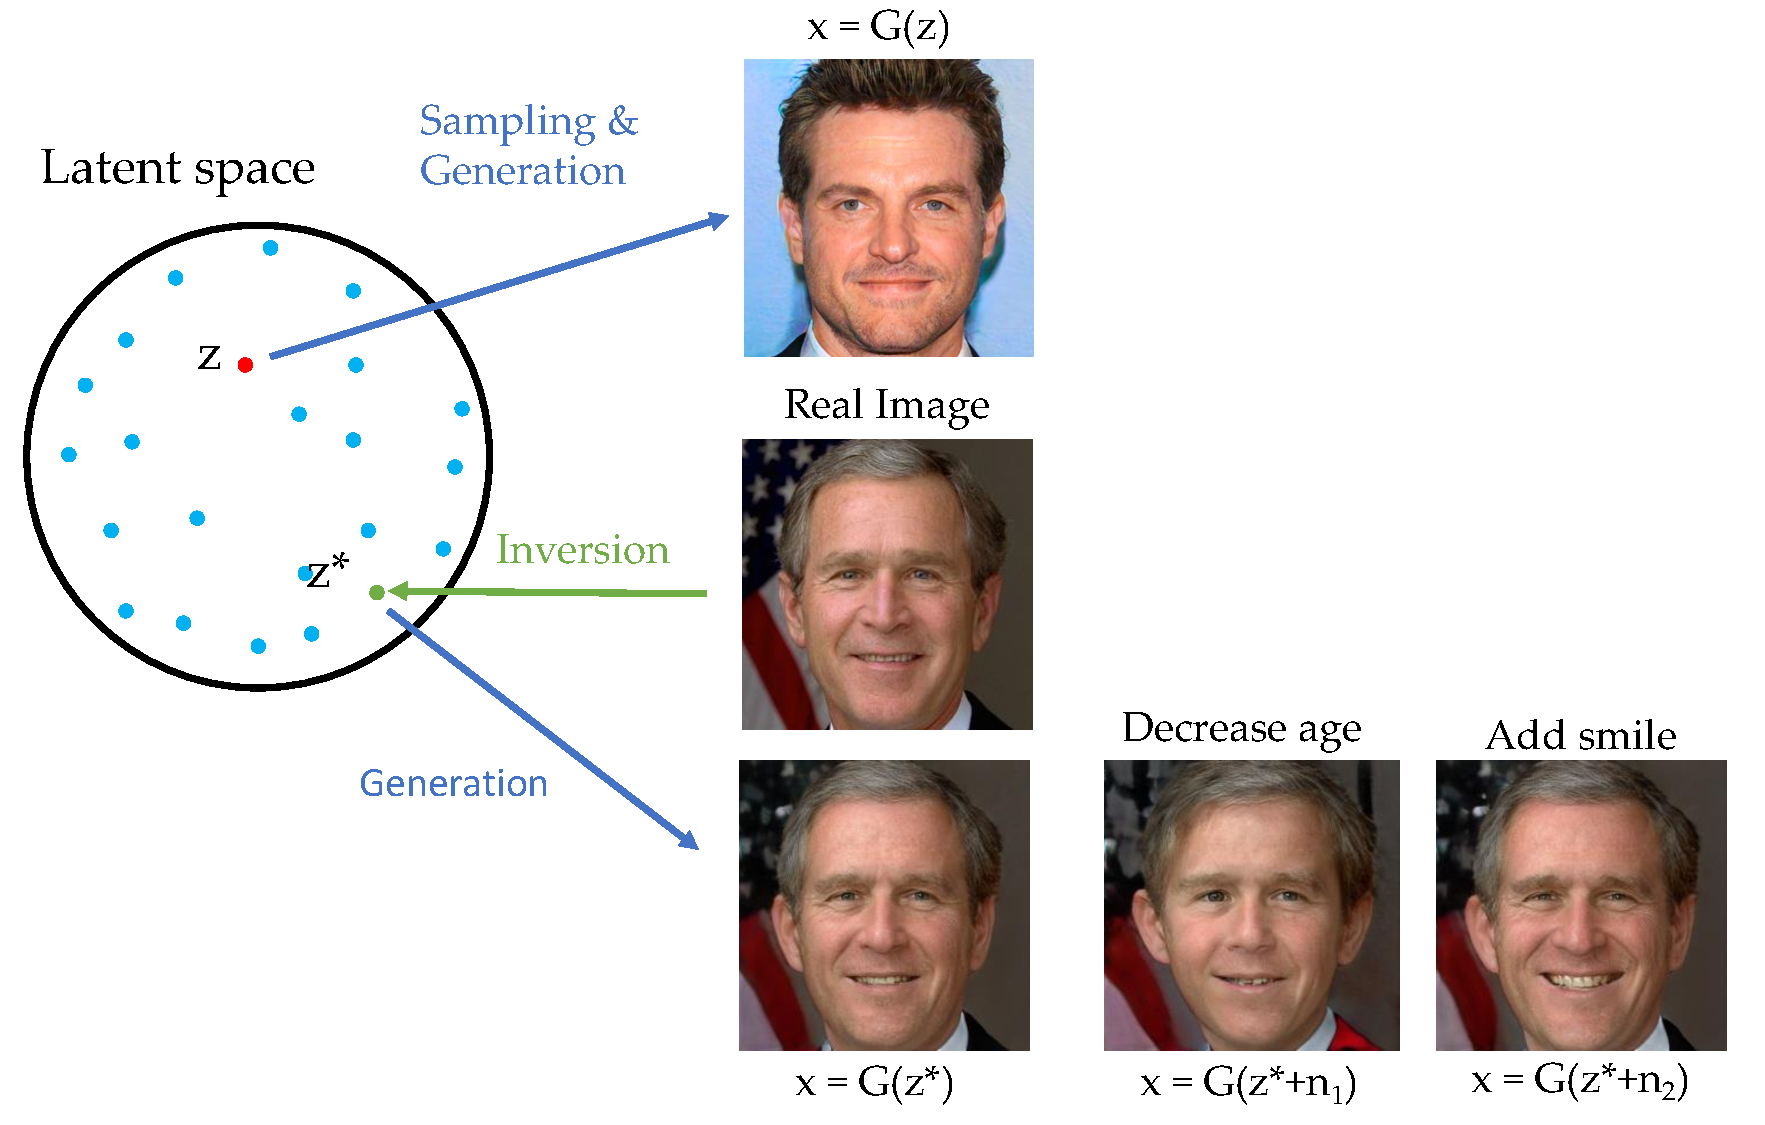
\includegraphics[width=0.9\linewidth]{images/overview_zhou}
\end{center}
\caption{\textbf{Illustration of GAN inversion.} Different from the conventional sampling and generation process using trained generator $G$, GAN inversion maps a given real image $x$ to the latent space and obtains the latent code $\mathbf{z^{*}}$. The reconstructed image $x^{*}$ is then obtained by $x^*=G(\mathbf{z^{*}})$. By varying the latent code $\mathbf{z^{*}}$ in different interpretable directions \eg, $\mathbf{z^{*}}+\mathbf{n_1}$ and $\mathbf{z^{*}}+\mathbf{n_2}$ where $\mathbf{n_1}$ and $\mathbf{n_2}$ model the age and smile in the latent space respectively, we can edit the corresponding attribute of the real image. The reconstructed results are from \cite{zhu2020indomain}.
}
\label{fig:overview}
\end{figure}
}

\newcommand{\figtype}{
\begin{figure}[tbp]
\begin{center}
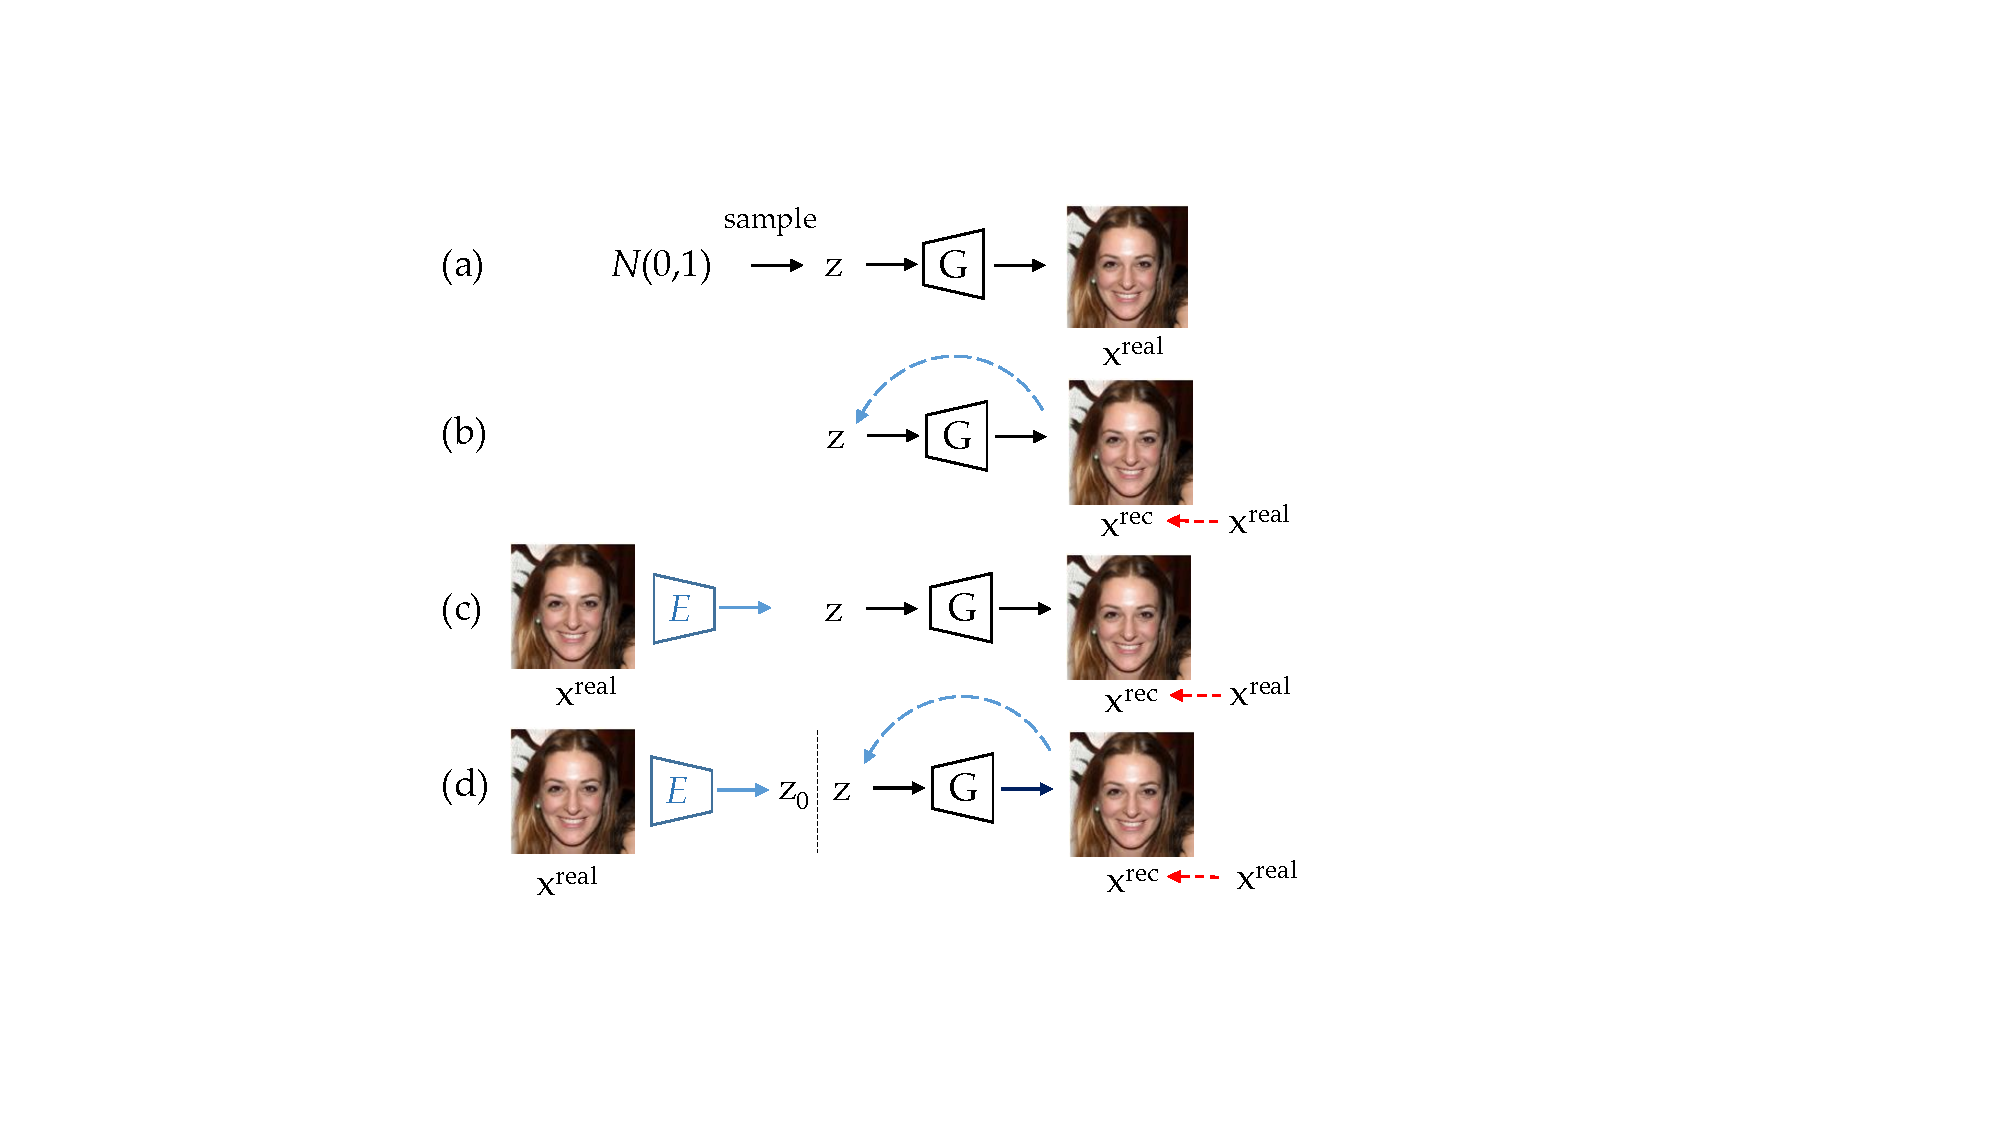
\includegraphics[width=0.95\linewidth]{images/inversion_types}
\end{center}
\caption{\textbf{Illustration of GAN Inversion Methods.} 
(a) given a well-trained GAN model, photo-realistic images can be generated from randomly sampled latent vectors. 
(b) {\bf optimization-based} inversion uses an optimization algorithm to iteratively optimize the latent code to minimize the pixel-wise reconstruction loss. 
(c) {\bf learning-based} inversion builds an encoder network that maps an image into the latent space. 
(d) {\bf hybrid} approach uses the encoder to generate an initialization for optimization, \ie, an encoder network is first used to obtain an approximate embedding and then refine it with an optimization algorithm.}
\label{fig:inversion_types}
\end{figure}
}

\newcommand{\figwalk}{
\begin{figure}[t]
\centering
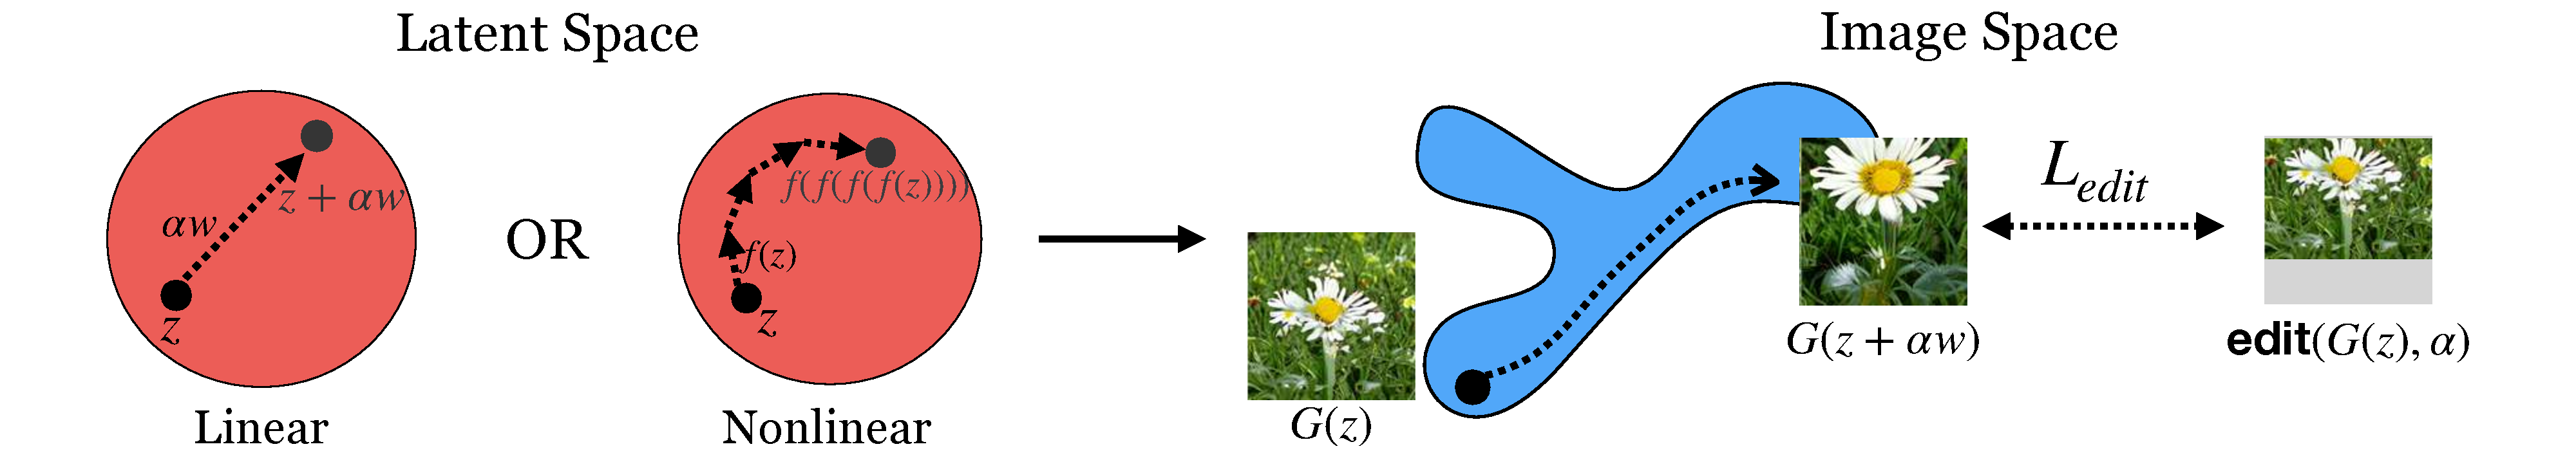
\includegraphics[width=1\columnwidth]{images/walk.pdf}
\caption{Illustration of discovering interpretable directions in the latent space~\cite{jahanian2020steerability}. 
The goal is to find a path in $\mathcal{Z}$ space to transform the generated image $G(\mathbf{z})$ to its edited version $\texttt{edit}(G(\mathbf{z},\alpha))$, \eg, an $\alpha \times$ zoom. 
The transformation can be represented as $G(\mathbf{z}+\alpha \mathbf{w})$ for a linear walk or $G(f(f(...(\mathbf{z})))$ for a non-linear walk.}
\label{fig:walk}
\end{figure}
}

\newcommand{\figindomain}{
\begin{figure}[tbp]
\begin{center}
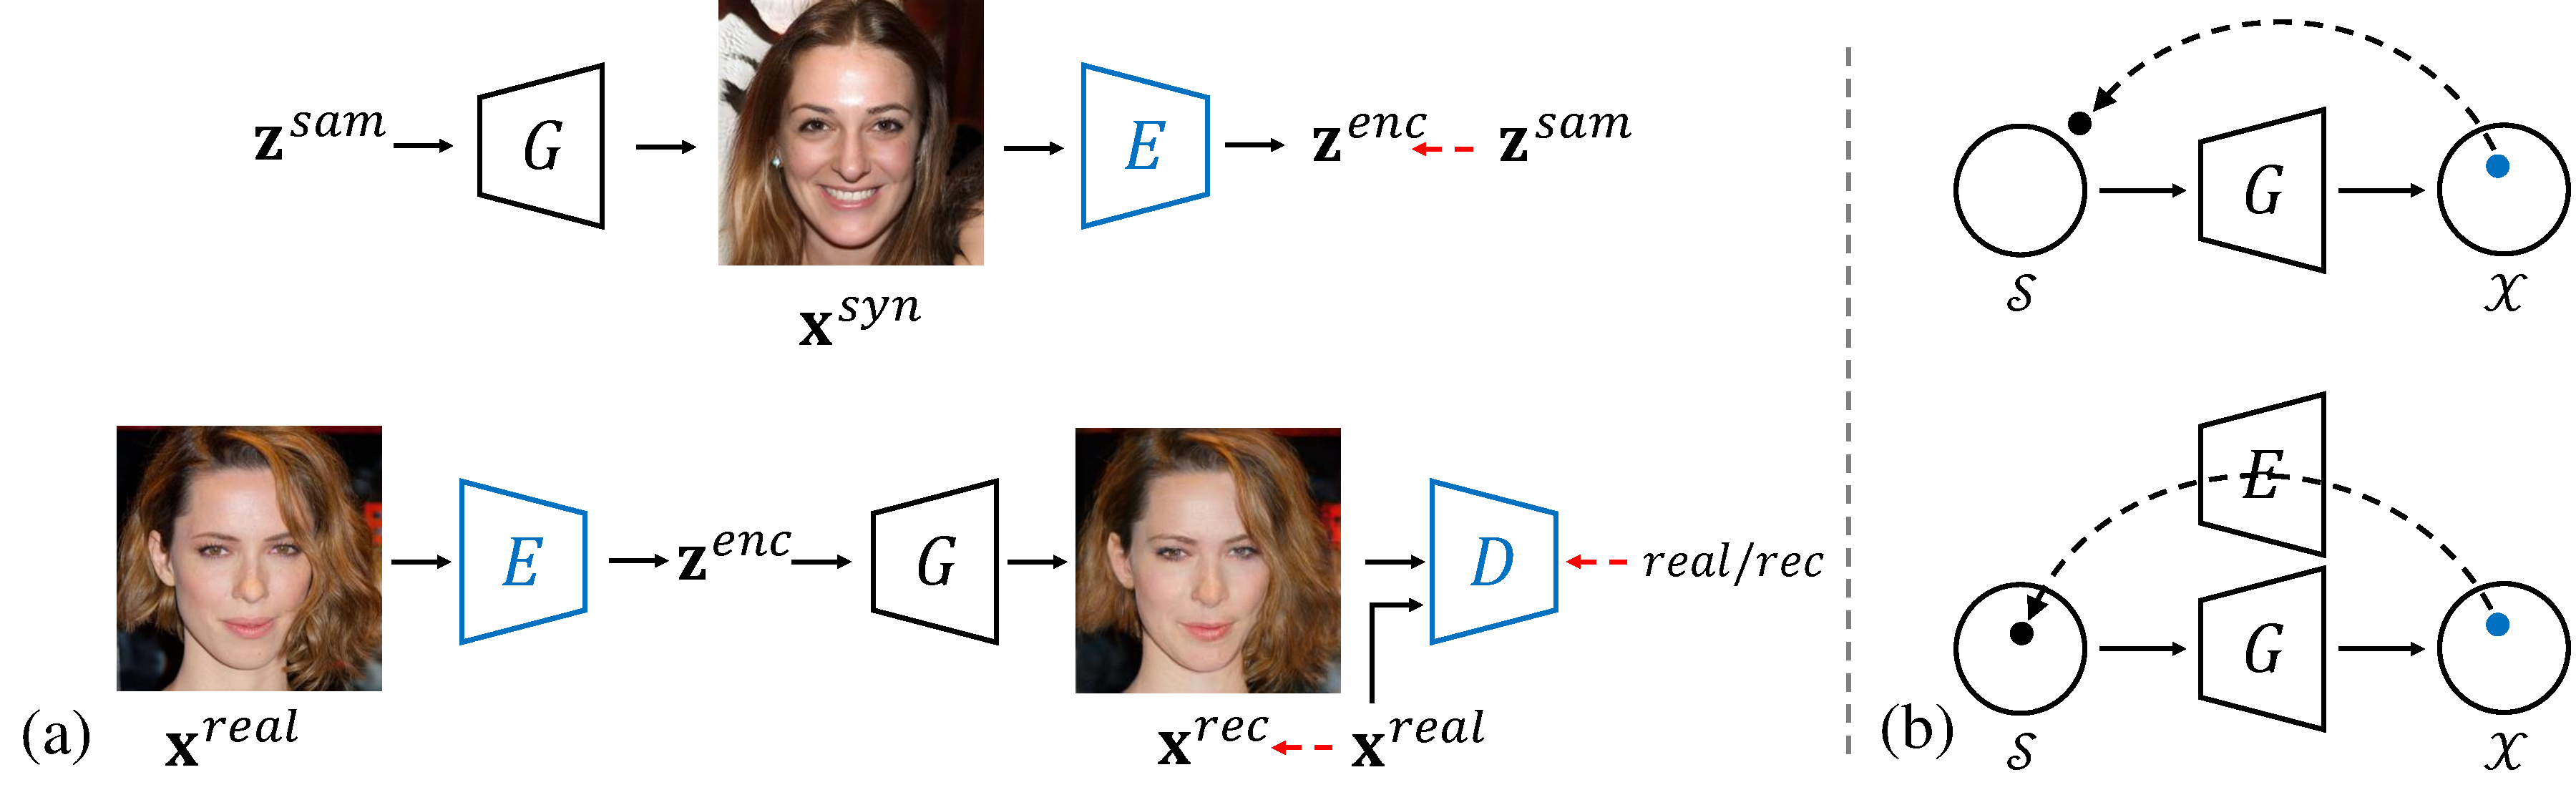
\includegraphics[width=0.95\linewidth]{images/indomain_comp.pdf}
\end{center}
\caption{\textbf{Comparisons between the training of (upper) conventional encoder and (lower) domain-guided encoder proposed in~\cite{zhu2020indomain} for GAN inversion.} Blue blocks represent trainable models and red dashed arrows indicate the supervisions. The domain-guided encoder is trained to recover the real images, instead of being trained with synthesized data to recover the latent code. The generator $G$ is well-trained with fixed weights during training $E$. (b) The comparison between the conventional optimization and the domain-regularized optimization proposed in~\cite{zhu2020indomain}. The well-trained domain-guided encoder $E$ is involved as a regularization to fine-tune the latent code in the semantic domain during $\mathbf{z}$ optimization.}
\label{fig:indomain}
\end{figure}
}

\newcommand{\fignoninference}{
\begin{figure}[tbp]
\begin{center}
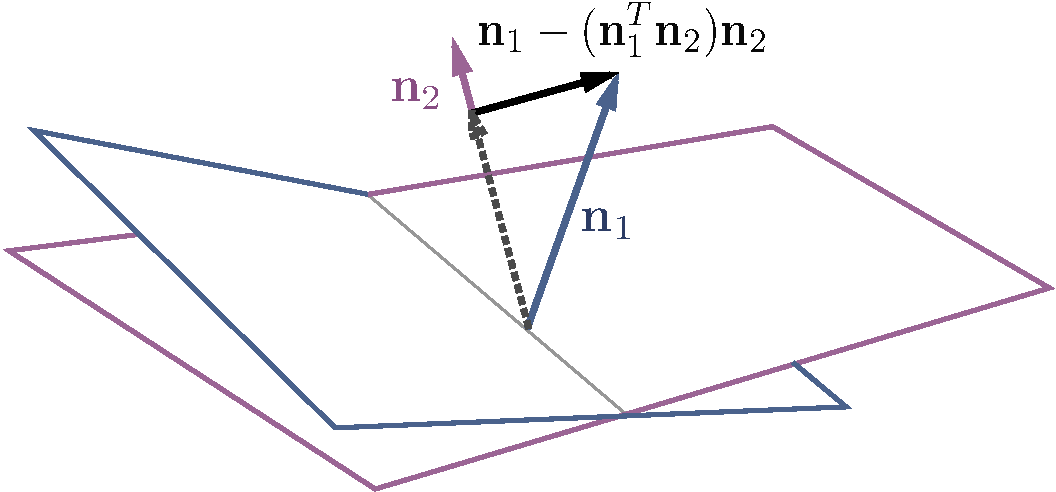
\includegraphics[width=0.6\linewidth]{images/projection}
\end{center}
\caption{\textbf{Illustration of the non-interference property in subspace.} The projection of $\mathbf{n}_{1}$ onto $\mathbf{n}_{2}$ is subtracted from $\mathbf{n}_{1},$ resulting in a new direction $\mathbf{n}_{1}-(\mathbf{n}_{1}^{\top} \mathbf{n}_{2}) \mathbf{n}_{2}$. This figure is from~\cite{shen2020interpreting}.}
\label{fig:projection}
\end{figure}
}

\newcommand{\figroi}{
\begin{figure}[tbp]
\centering
%\vspace{-0.5cm} 
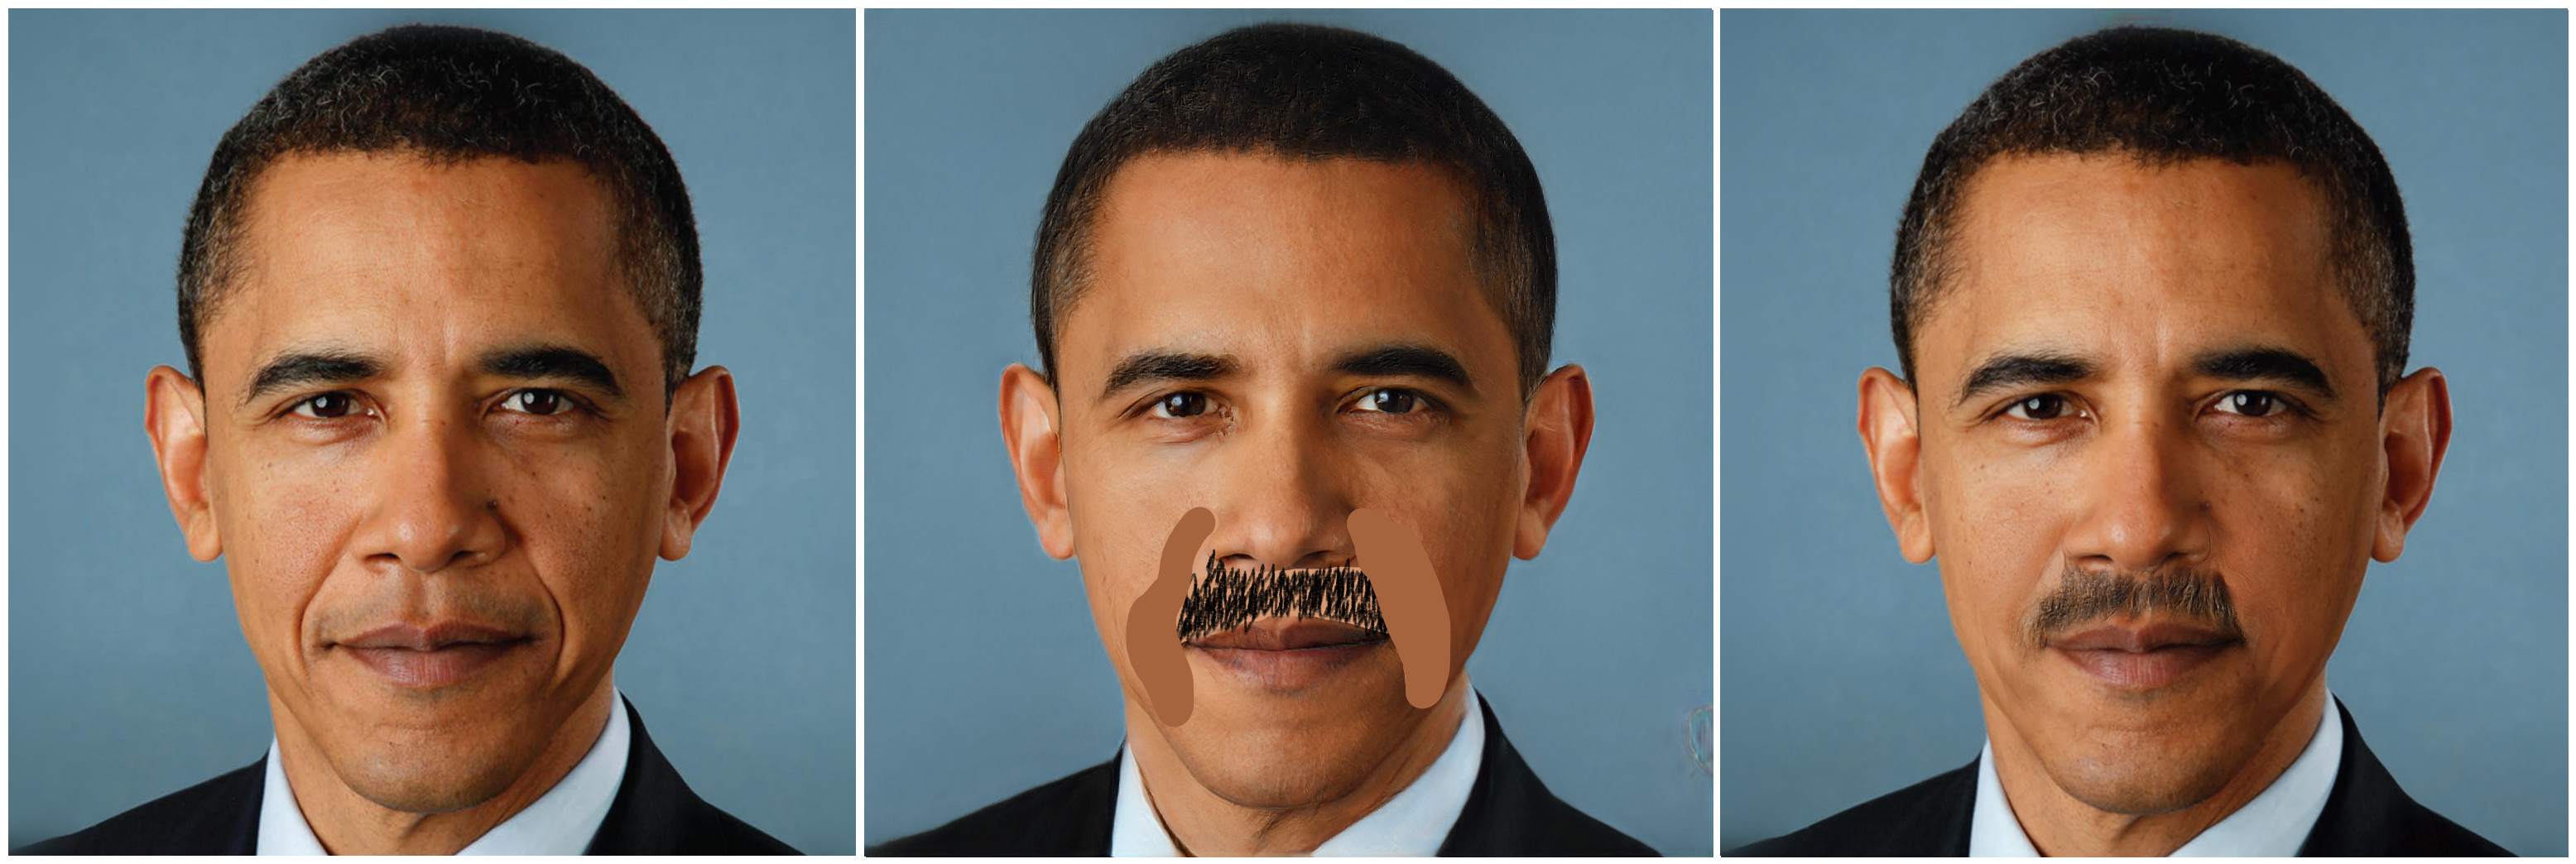
\includegraphics[width= 0.95\linewidth]{images/local_obama.jpg}
 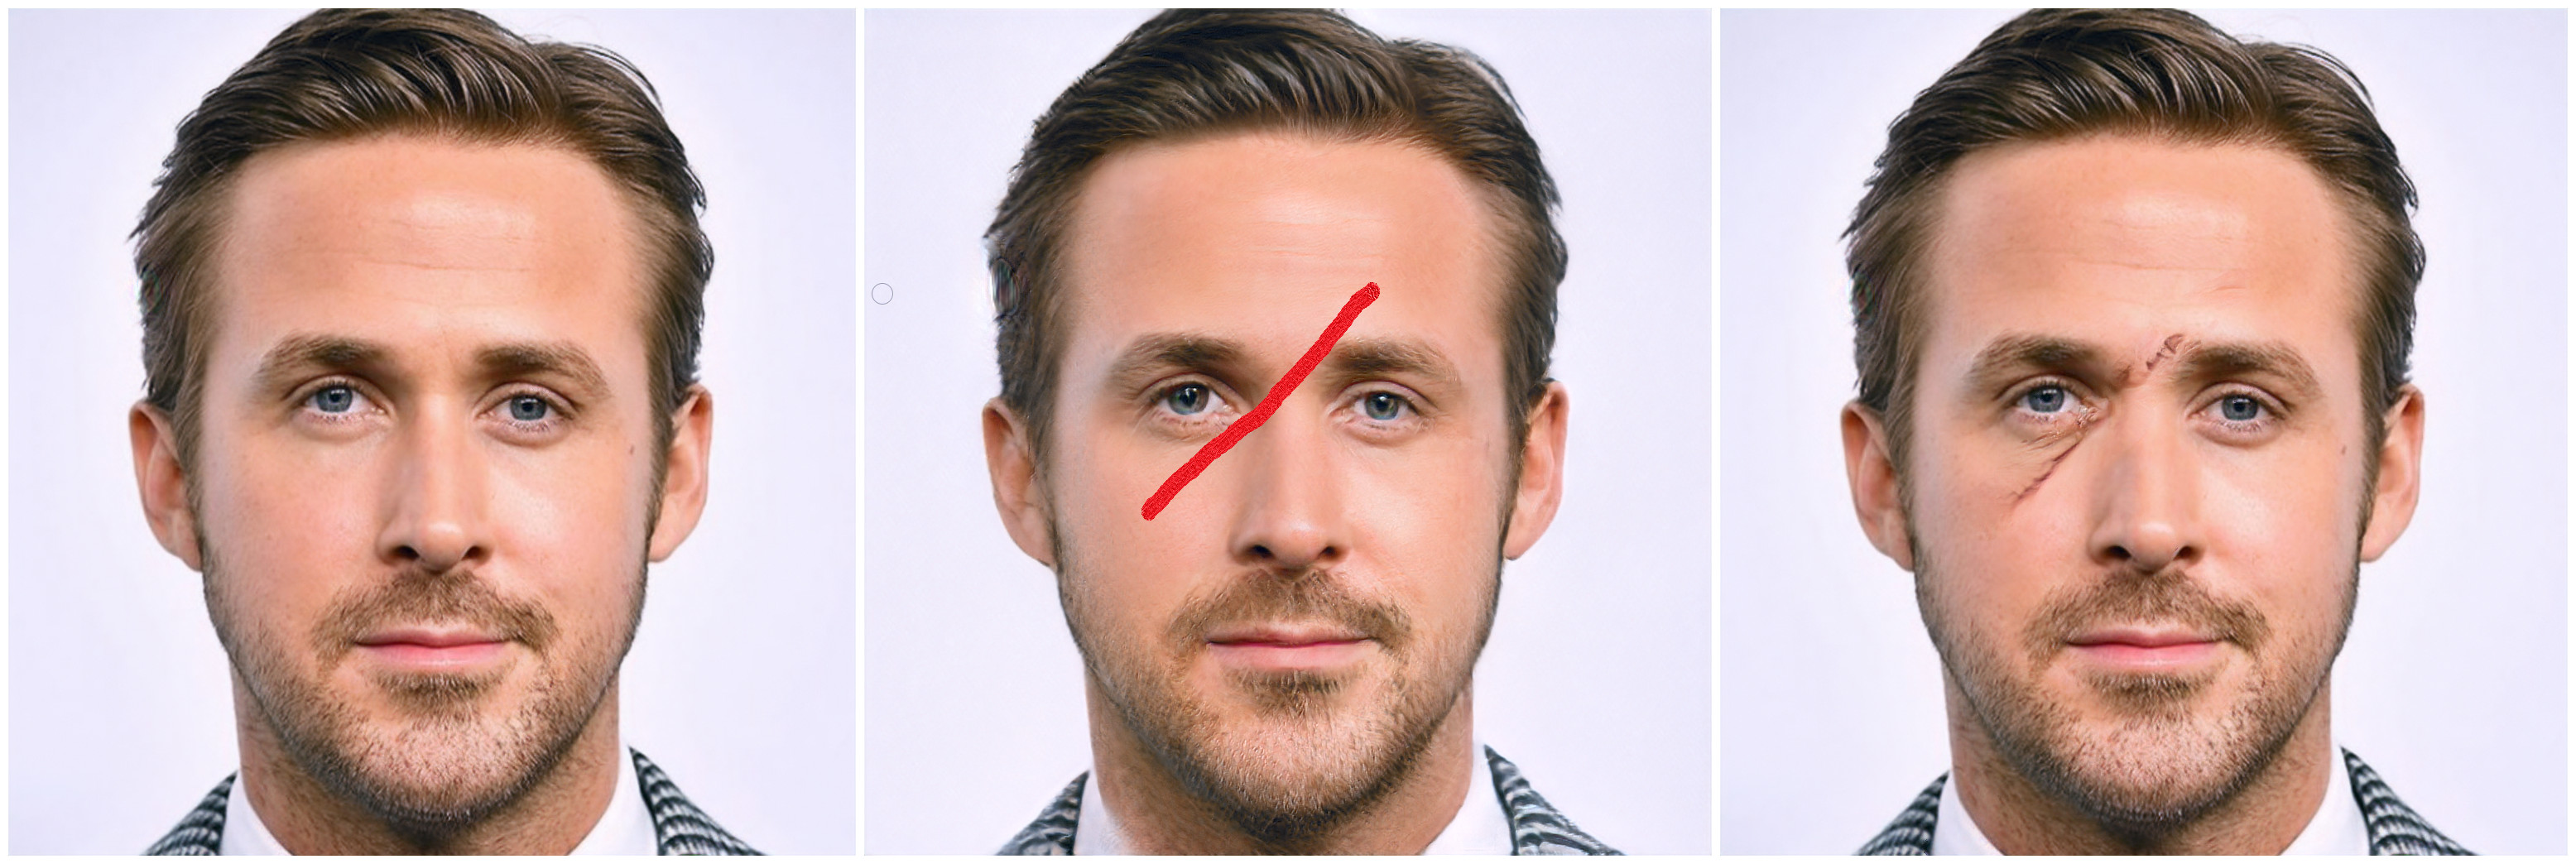
\includegraphics[width=0.95\linewidth]{images/local_ryan.jpg}
\caption{\textbf{Illustration of region-of-interest editing~\cite{abdal2020image2stylegan2}.} From left to right: base image; scribbled image; result of local edits.}
\label{fig:local}
\end{figure}
}

\newcommand{\figrewrite}{
\begin{figure}[tbp]
\begin{center}
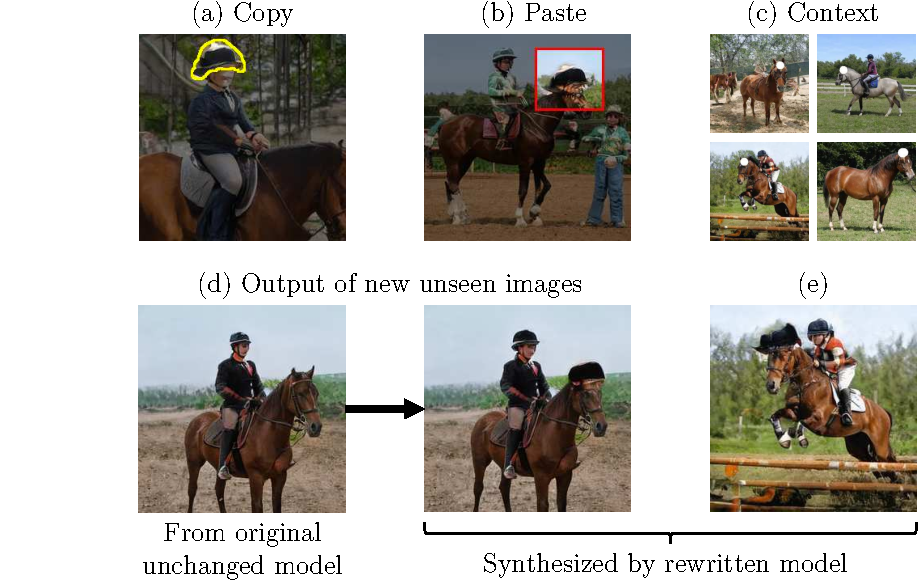
\includegraphics[width=0.95\linewidth]{images/ganrewriting}
\end{center}
\caption{\textbf{Copy-Paste-Context interface for rewriting a model~\cite{zhu2016generative}.} 
%The first row is the user inputs and the last are corresponding model outputs. 
(a) Copy: the user uses a brush to select a region containing an interesting object or shape, defining the target. (b) Paste: The user positions and pastes the copied object into a single target image. (c) Context: To control generalization, the user selects target regions in several images. (d) The edit is applied to the model, not to a specific image, such that newly generated images will have hats on top of horse heads. (e) The change has been applied to different types of horses and poses.}
\label{fig:ganrewriting}
\end{figure}
}

\newcommand{\figood}{
\begin{figure}[tbp]
\begin{center}
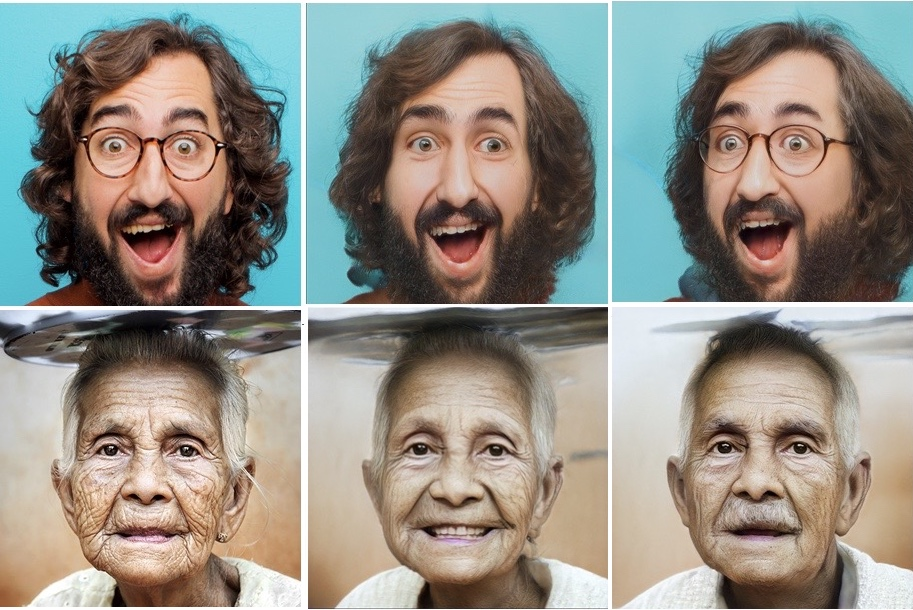
\includegraphics[width=0.95\linewidth]{images/ood}
\end{center}
\caption{\textbf{Illustration of face image manipulation.} These are real image editing results from using StyleFlow~\cite{abdal2020styleflow}.}
\label{fig:ood}
\end{figure}
}

\newcommand{\figapp}{
\begin{figure}[tbp]
\begin{center}
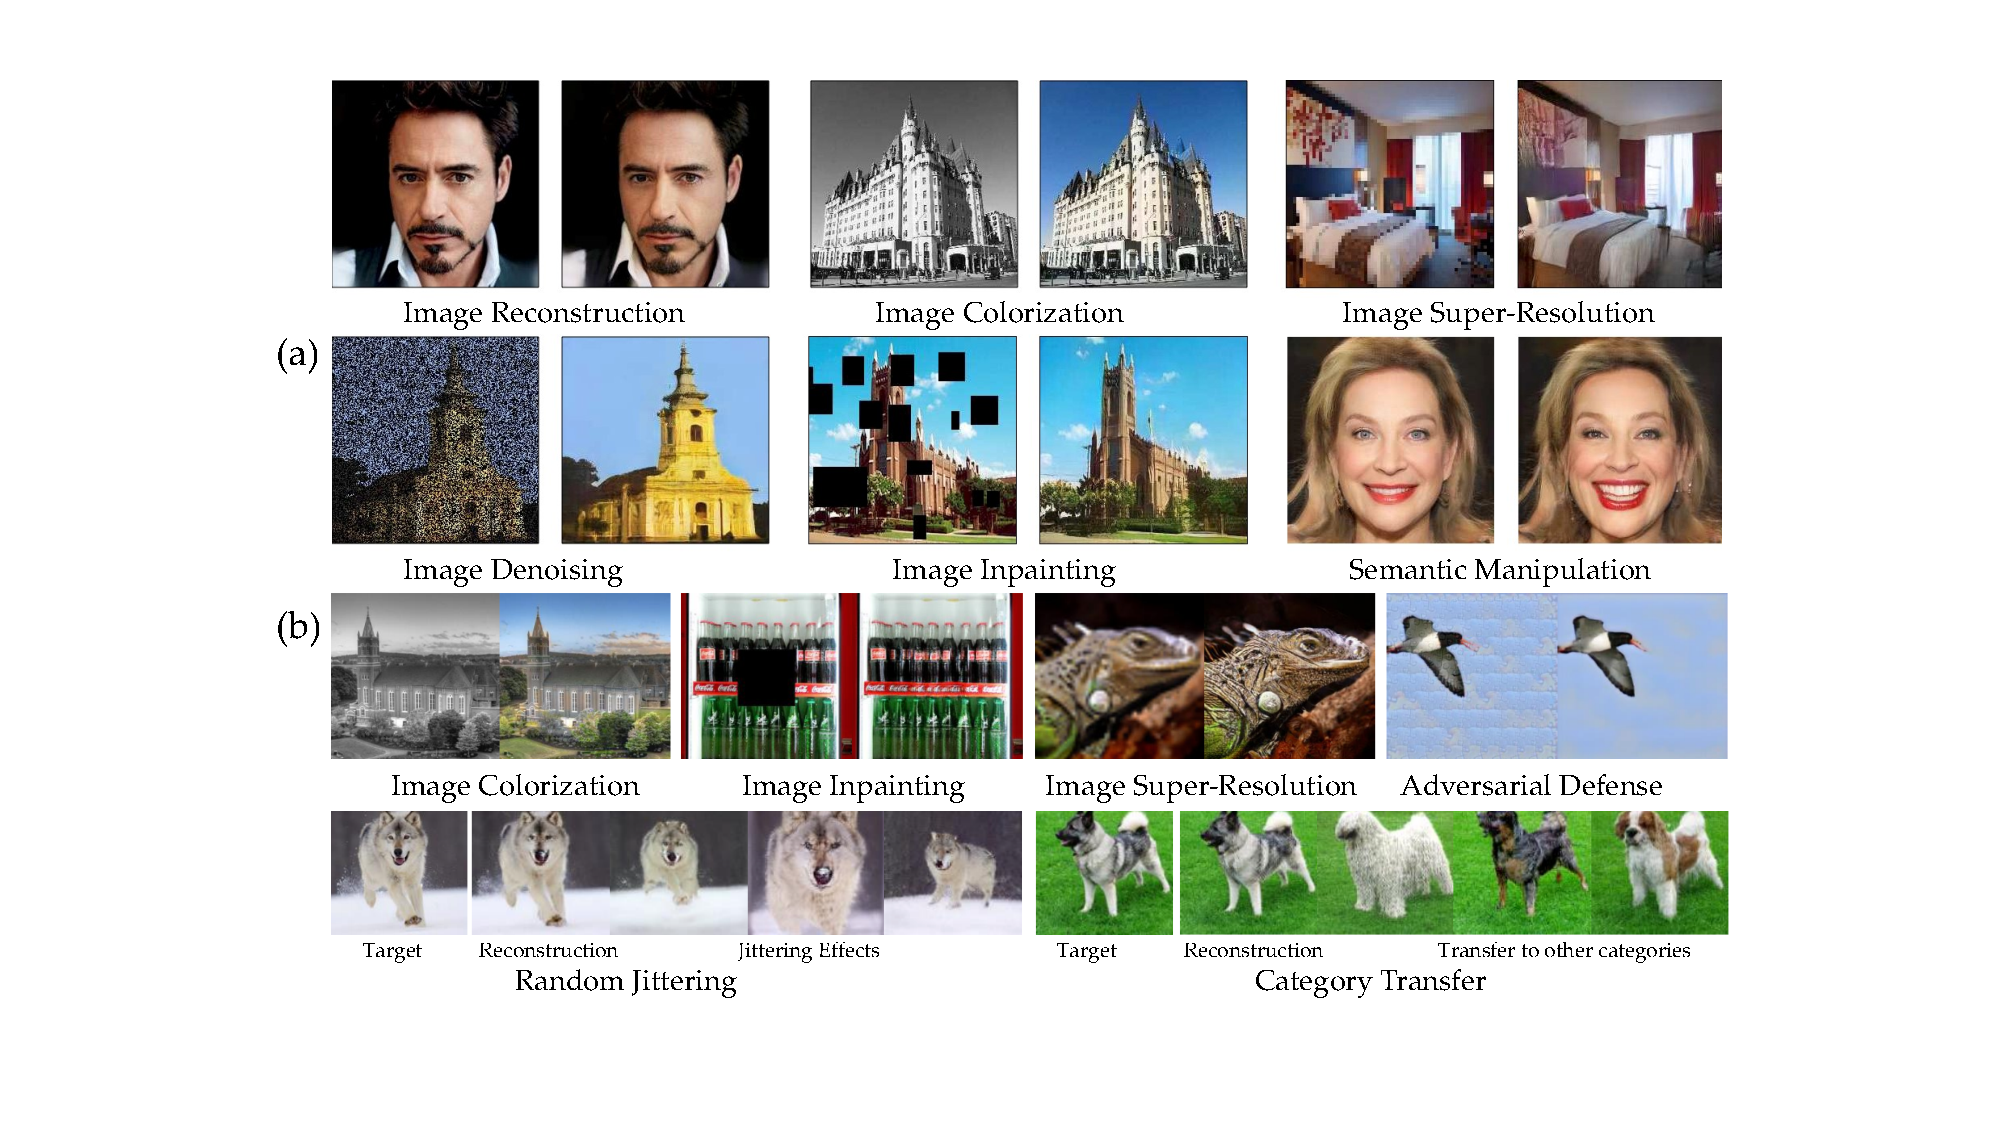
\includegraphics[width=0.95\linewidth]{images/application_zhou}
\end{center}
\caption{\textbf{Illustration of image processing using GAN inversion.}
GAN inversion does not require task-specific dense-labeled datasets and can be applied to many tasks like image reconstruction, image restoration and image manipulation. 
% GAN inversion does not require task-specific dense-labeled datasets and can be applied to many tasks like image reconstruction (a), image restoration (b)(c)(d)(e) and image manipulation (f). 
The upper illustration (a) is from mGANPrior~\cite{gu2020image} and the lower (b) is from DGP~\cite{pan2020exploiting}.}
\label{fig:application}
\end{figure}
}

\newcommand{\figcorrect}{
\begin{figure}[tbp]
\begin{center}
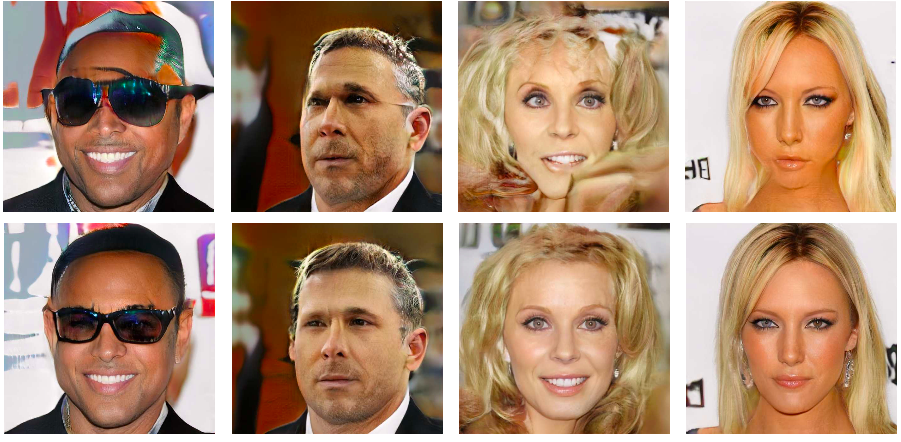
\includegraphics[width=0.98\linewidth]{images/correction}
\end{center}
\caption{\textbf{Results of artifacts correction.}  First row shows are examples generated by PGGAN~\cite{karras2017progressive}. The second row presents the gradually corrected synthesis by moving the latent codes along the positive quality direction. This figure is from~\cite{shen2020interpreting}.}
\label{fig:correction}
\end{figure}
}

\newcommand{\algotransfer}{
\begin{algorithm}[t]
\SetAlgoLined
\KwIn{images $x, y \in \mathbb{R}^{n \times m \times 3}$; masks $M_b$}
\KwOut{the embedded code $(\mathbf{w_o},\mathbf{n_o})$} 
$(\mathbf{w^*},\mathbf{n_i}) \leftarrow$ initialize()\;
{$\mathbf{w_o} = W_{l}(M_b,M_b,1 ,\mathbf{w^*},\mathbf{n_i},x)$\
$+ M_{st}(1-M_b,\mathbf{w^*} ,\mathbf{n_i}, y)$\;
$\mathbf{n_o} = {Mk}_{n}(M_b,\mathbf{w_o},\mathbf{n_i},x,G(\mathbf{w_o}))$\;
}
\caption{Local style transfer~\cite{abdal2020image2stylegan2}}
\label{alg:local_style_tranfer}
\end{algorithm}
}

\newcommand{\figtransfer}{
\begin{figure}[tp]
\centering
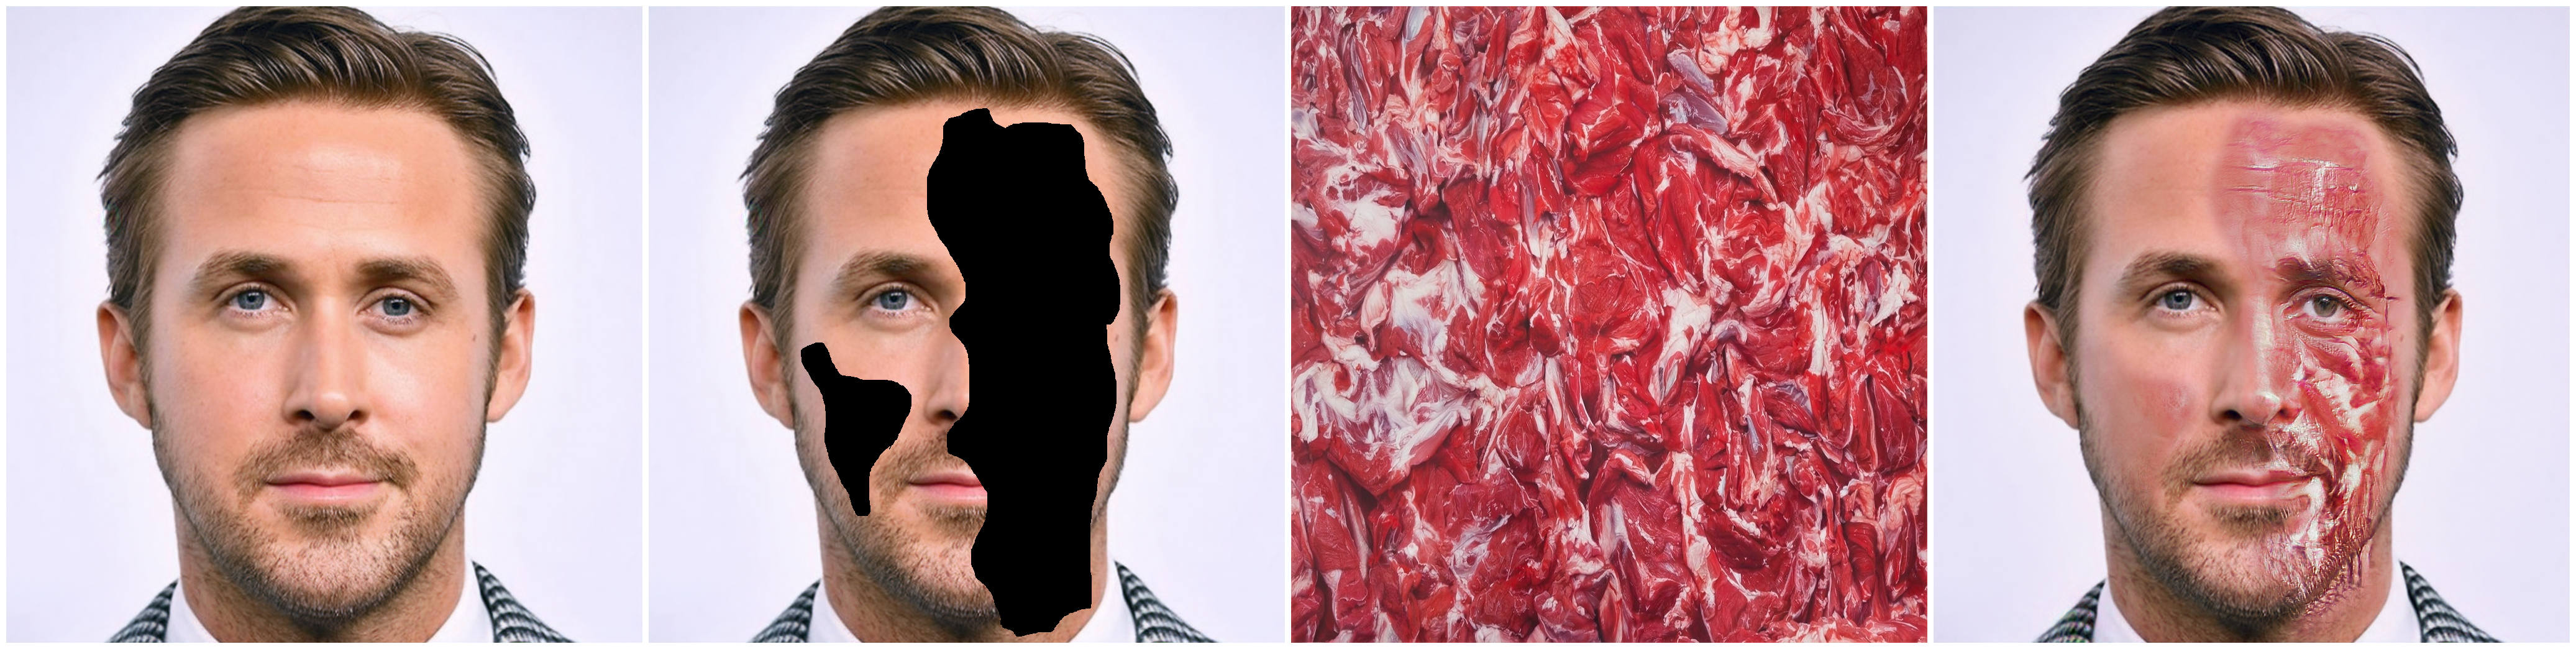
\includegraphics[width=0.95\linewidth]{images/style_ryan.jpg}
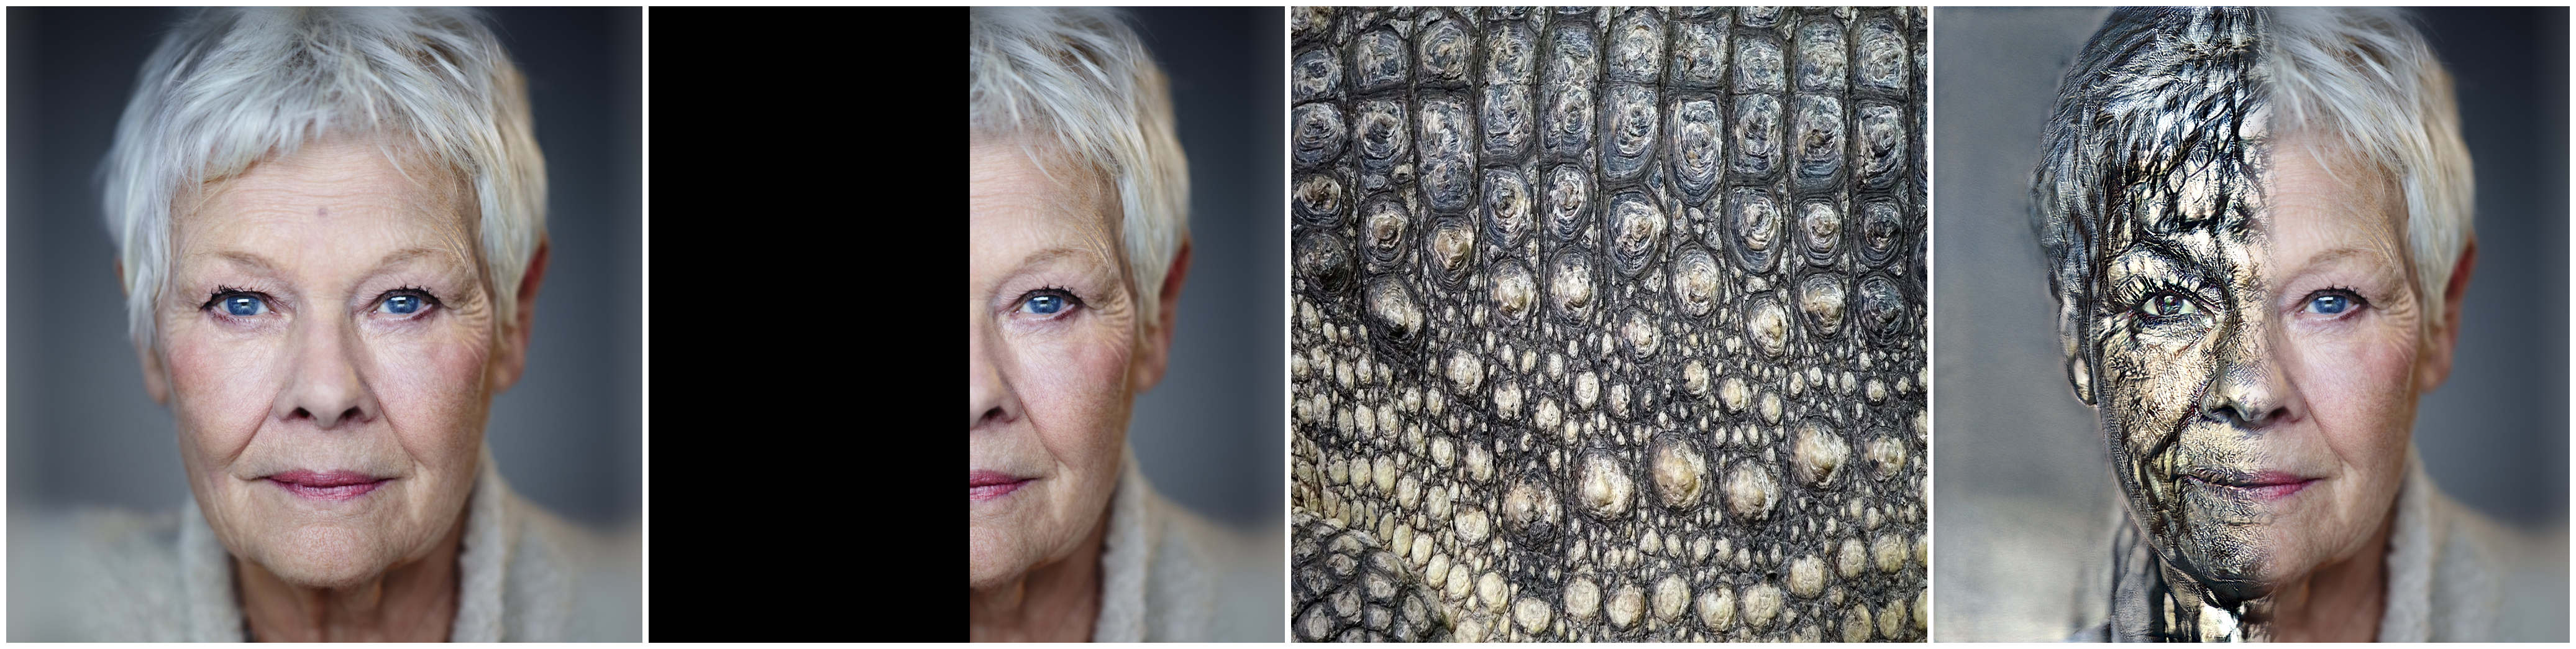
\includegraphics[width=0.95\linewidth]{images/style_judi.jpg}
\caption{\textbf{Illustration of local style transfer~\cite{abdal2020image2stylegan2}.} From left to right: base image, masked region, style image, local style transfer result.}
\label{fig:local_style_tranfer}
\end{figure}
}

\newcommand{\figinteractive}{
\begin{figure}[tbp]
\begin{center}
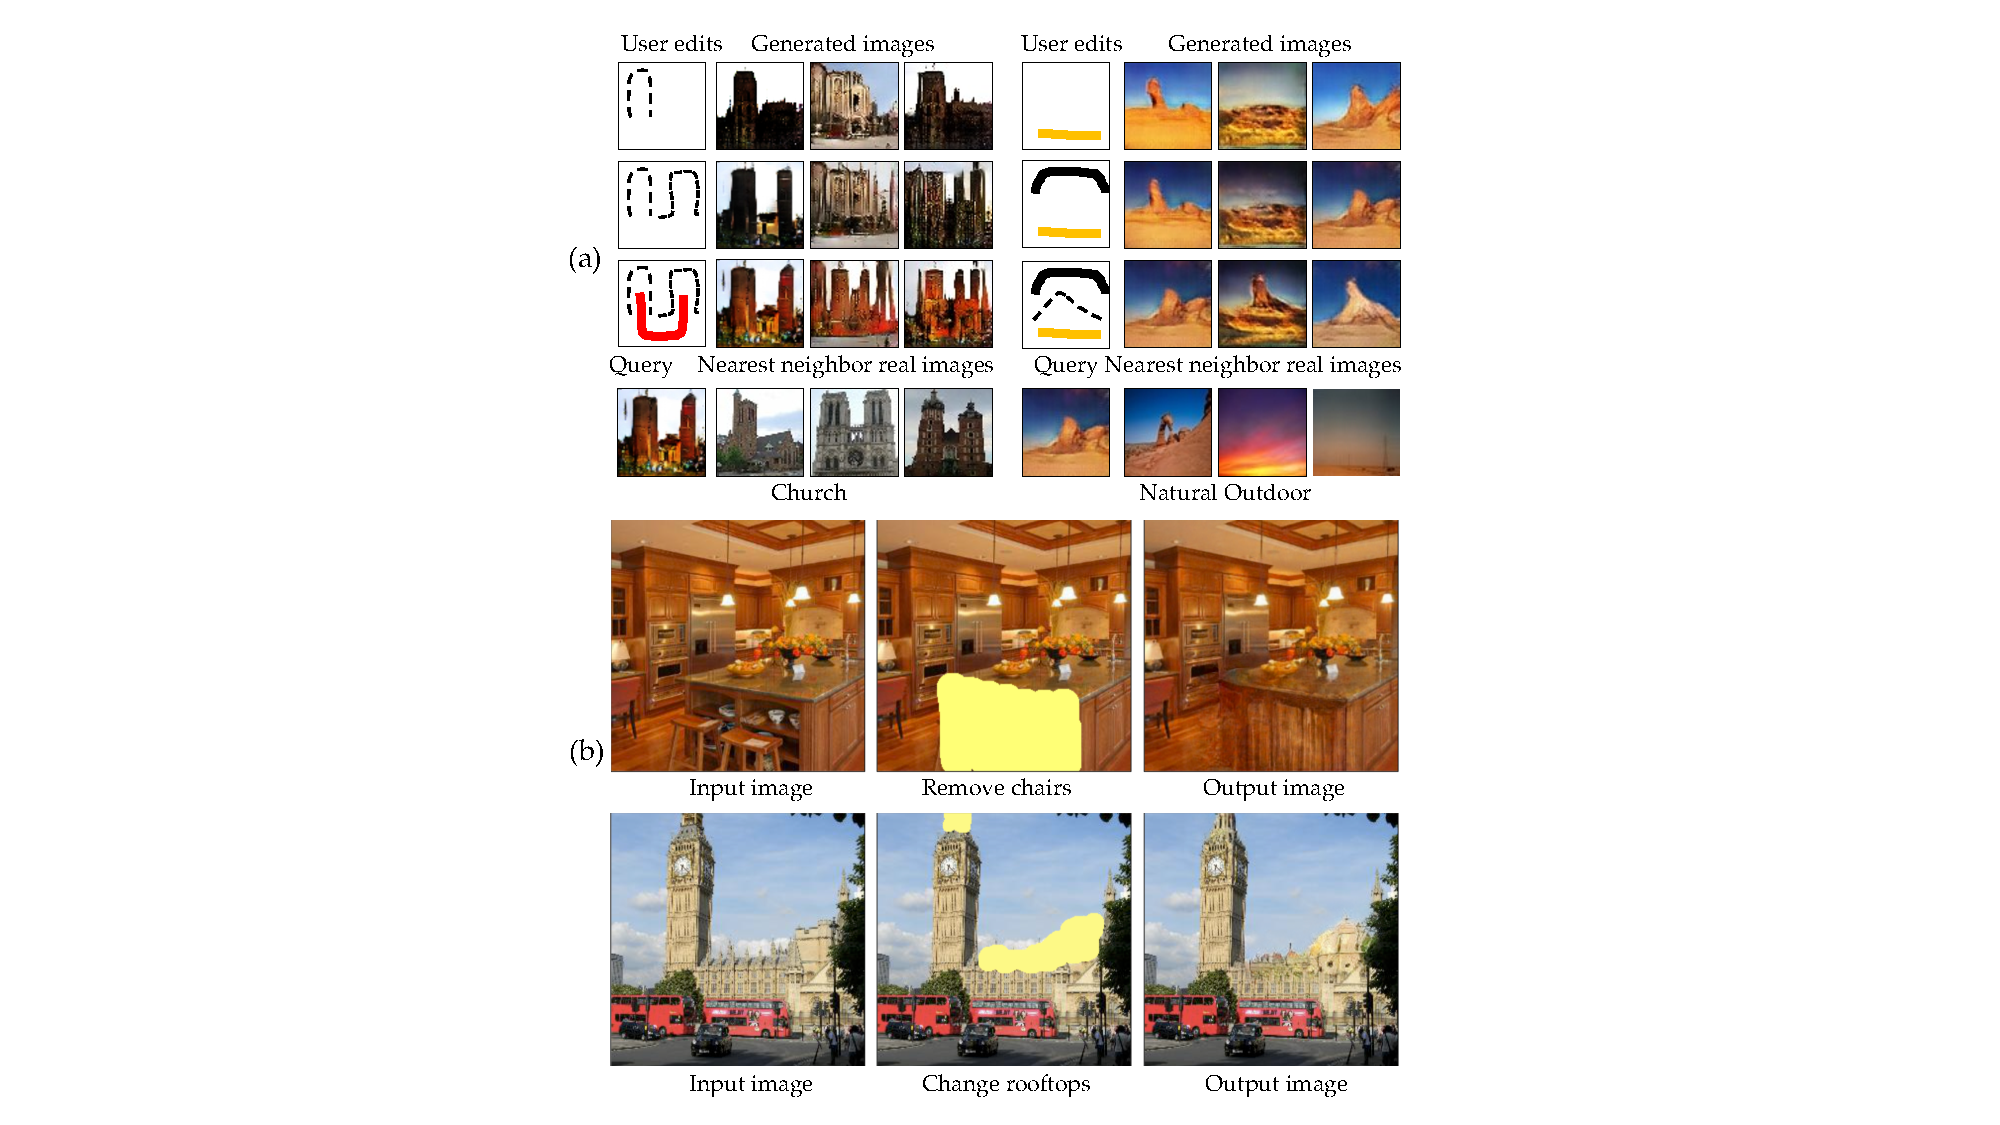
\includegraphics[width=0.95\linewidth]{images/interactive}
\end{center}
\caption{\textbf{Illustration of interactive image generation using GAN inversion.} (a) illustrates results from ~\cite{zhu2016generative}. The users are allowed to use the brush tools to generate an image from scratch and keep adding more scribbles or sketches for refinement. The last row shows the most similar real images to the generated images. Dashed line represents the sketch tool, and color scribble means the color brush.
(b) is from GANPaint~\cite{bau2019ganpaint}. The brushes can draw semantically meaningful units like removing chairs or adding rooftops.
}
\label{fig:interactive}
\end{figure}
}

\newcommand{\figdiffusion}{
\begin{figure}[tbp]
\begin{center}
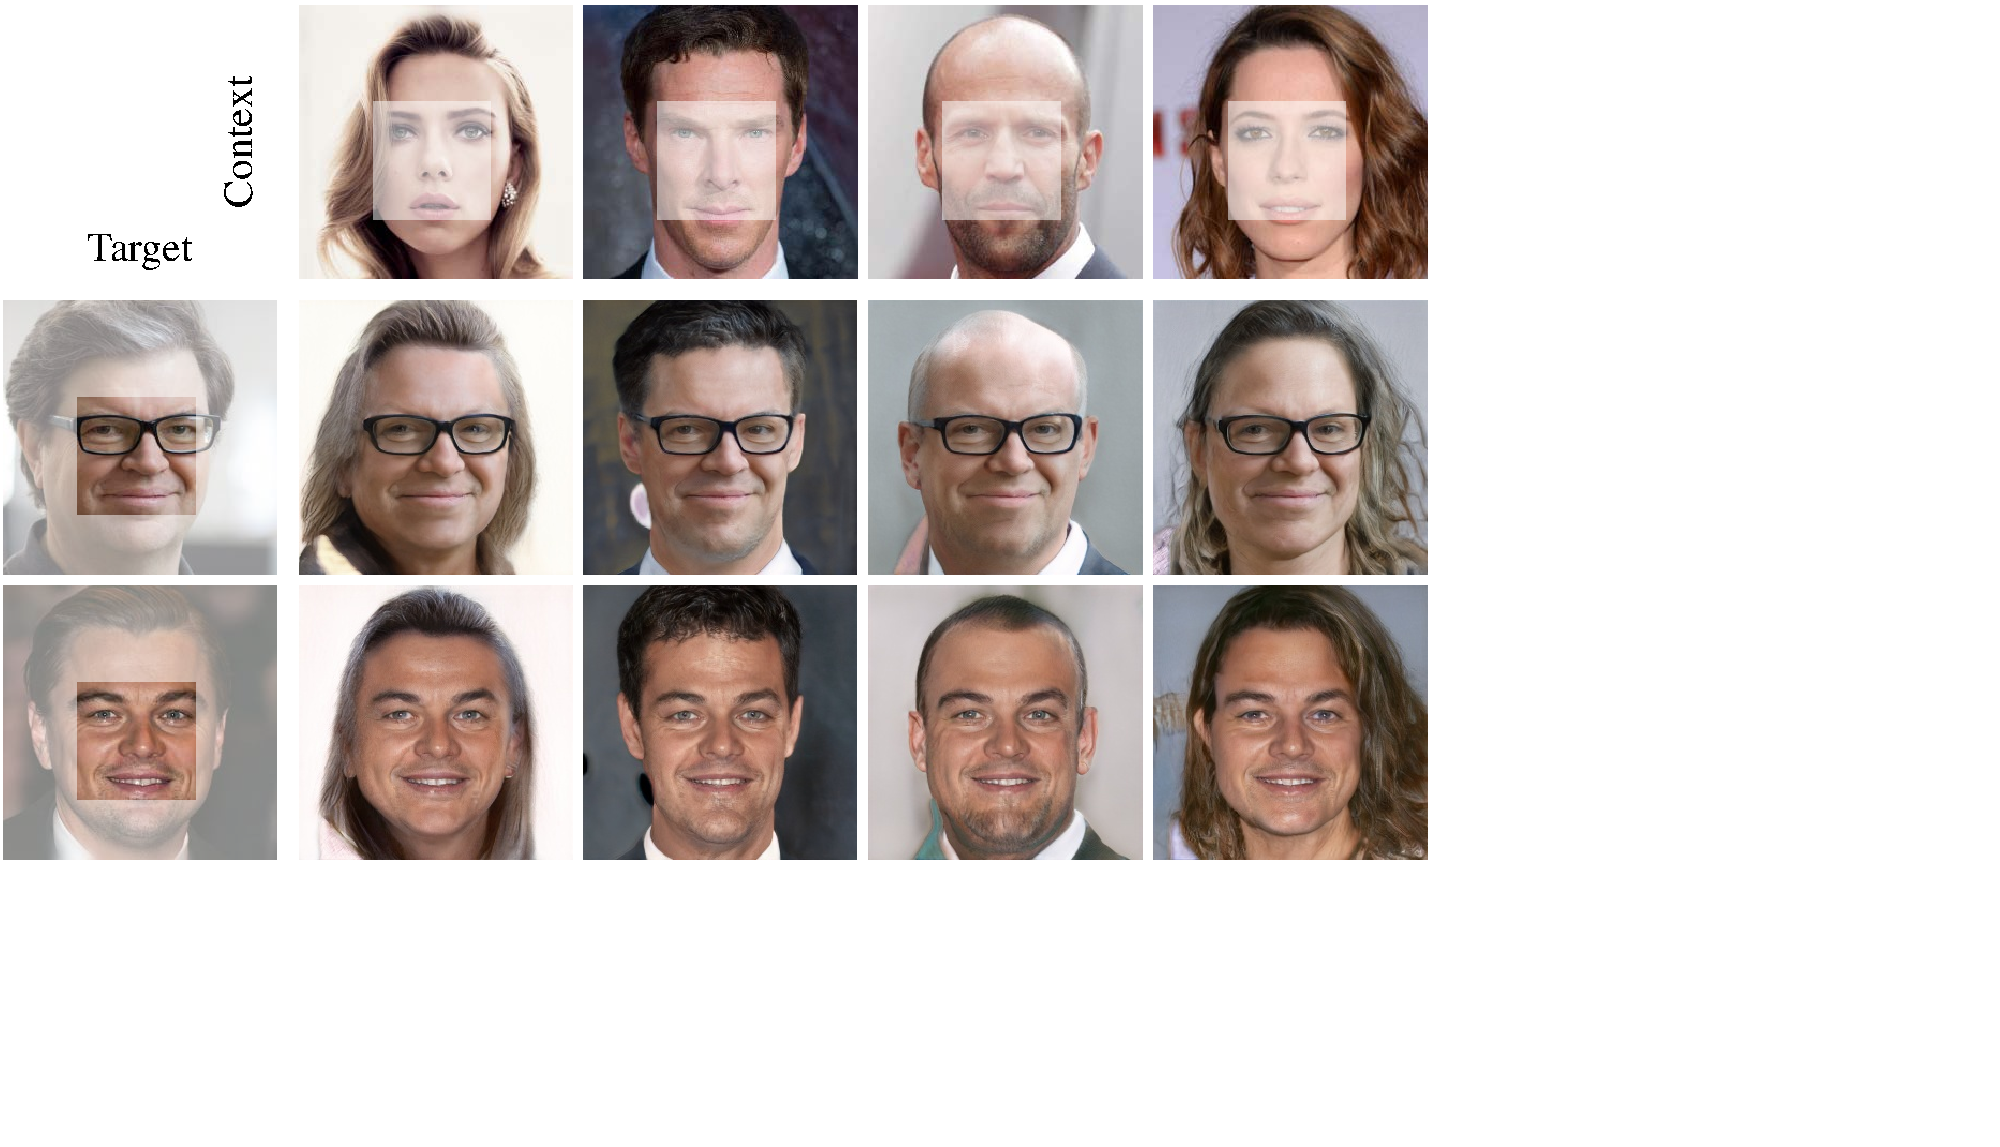
\includegraphics[width=0.95\linewidth]{images/diffusion.pdf}
\end{center}
\caption{\textbf{Semantic diffusion results using the in-domain GAN inversion method~\cite{zhu2020indomain}}. Target images in the first column are naturally diffused into context images in the first row with the identify preserved.}
\label{fig:diffusion}
\end{figure}
}

\newcommand{\tabfeature}{
\begin{table*}[htbp]
\caption{Characteristics of GAN inversion methods. `Type' includes Learning-based (L.), Optimization-based (O.), Hybrid (H.), and Closed-Form (C.) GAN inversion. I.-D., S.-A., L.-W., N.-I., R.-I. and O.-D. denote discovering the Interpretable Directions in a Supervised (S.) or an Unsupervised (U.) manner, Semantic-Aware, Layer-Wise, Non-Interference, Region-of-Interest, and Out-of-Distribution, respectively. GAN model and Dataset indicate which Pretrained Models are trained on which Dataset that a method is inverting, which can be found in Section~\ref{sec:model_data}.}
\label{tab:taxonomy}
\begin{center}
\scalebox{0.92}{
\begin{tabular}{c|c|c|c|c|c|c|c|c|c|c}
\toprule
Method  & Publication & Type &I.-D. &S.-A. &L.-W. &N.-I. &R.-I. &O.-D. &GAN Model & Dataset \\\hline
Zhu~\etal~\cite{zhu2016generative} &2016, ECCV &H. &\nxmark &\nxmark &\nxmark &\nxmark &\nxmark &\nxmark &\cite{radford2016dcgan} &\cite{yu2014local,zhou2014places,yu2015lsun}\\
Creswell~\etal~\cite{creswell2018inverting} &2018, TNNLS &O. &\nxmark &\nxmark &\nxmark &\nxmark &\nxmark &\nxmark &\cite{radford2016dcgan,gulrajani2017improved} &\cite{yu2014local,liu2015faceattributes}\\
GAN Dissection~\cite{bau2019gandissect} &2019, ICLR &O. &\nxmark &\ncmark &\ncmark &\nxmark &\ncmark &\nxmark &\cite{karras2017progressive} &\cite{yu2015lsun}\\
GAN Paint~\cite{bau2019ganpaint} & 2019, TOG &H. &\nxmark &\ncmark &\ncmark &\nxmark &\ncmark &\nxmark & \cite{karras2017progressive} & \cite{yu2015lsun}\\
Raj~\etal~\cite{raj2019gan} &2019, ICCV &O. &\nxmark &\nxmark &\nxmark &\nxmark &\nxmark &\nxmark &\cite{radford2016dcgan,zhang2019self} &\cite{yu2015lsun,lecun1998mnist,liu2015faceattributes}\\
GANSeeing~\cite{bau2019seeing} &2019, ICCV &H. &\nxmark &\ncmark &\ncmark &\nxmark & \nxmark &\nxmark &\cite{gulrajani2017improved,karras2017progressive,karras2019style}  &\cite{yu2015lsun}\\
Image2StyleGAN~\cite{abdal2019image2stylegan} &2019, ICCV &O. &\nxmark &\ncmark &\nxmark &\nxmark &\nxmark &\nxmark &\cite{karras2019style} &\cite{karras2019style} \\
Image2StyleGAN++~\cite{abdal2020image2stylegan2} &2020, CVPR &O. &\nxmark &\ncmark &\nxmark &\nxmark &\ncmark&\nxmark &\cite{karras2017progressive,karras2019style} &\cite{karras2017progressive,karras2019style}\\
mGANPrior~\cite{gu2020image} &2020, CVPR &O. &\nxmark &\ncmark &\ncmark &\ncmark &\nxmark &\ncmark &\cite{karras2017progressive,karras2019style} &\cite{karras2017progressive,karras2019style,yu2015lsun}\\
%IIN~\cite{esser2020invertible} &2020, CVPR &  &  &  &  &  &  &\\
Editing in Style~\cite{collins2020uncovering} &2020, CVPR &O. &\nxmark &\ncmark &\nxmark &\nxmark &\ncmark &\nxmark &\cite{karras2017progressive,karras2019style,karras2020analyzing} &\cite{karras2019style,yu2015lsun}\\
StyleRig~\cite{tewari2020stylerig} &2020, CVPR &L. &\nxmark &\ncmark &\nxmark &\nxmark &\nxmark &\nxmark &\cite{karras2019style} &\cite{karras2019style}\\
InterFaceGAN~\cite{shen2020interpreting} &2020, CVPR &L., O. &S. &\ncmark &\ncmark &\ncmark &\nxmark &\ncmark  &\cite{karras2017progressive,karras2019style} &\cite{karras2019style}\\
YLG~\cite{daras2020your} &2020, CVPR &O. &\nxmark &\nxmark &\nxmark &\nxmark &\nxmark &\ncmark &\cite{zhang2019self} &\cite{russakovsky2015imagenet}\\
GANRewriting~\cite{bau2020rewriting} &2020, ECCV &O. &\nxmark &\ncmark &\nxmark &\nxmark &\ncmark &\nxmark &\cite{karras2017progressive,karras2020analyzing} &\cite{yu2015lsun}\\
DGP~\cite{pan2020exploiting} &2020, ECCV &O. &\nxmark &\nxmark &\ncmark &\nxmark &\nxmark &\nxmark &\cite{brock2018large} &\cite{zhou2014places,russakovsky2015imagenet}\\
Huh~\etal~\cite{huh2020transforming} &2020, ECCV &O. &\nxmark &\ncmark &\nxmark &\nxmark &\ncmark &\ncmark &\cite{brock2018large,karras2020analyzing} &\cite{russakovsky2015imagenet,yu2015lsun,karras2019style}\\
IDInvert~\cite{zhu2020indomain} &2020, ECCV &H. &\nxmark &\ncmark &\nxmark &\nxmark &\nxmark &\ncmark &\cite{karras2019style}  &\cite{karras2019style,yu2015lsun}\\
StyleGAN2 Distillation~\cite{viazovetskyi2020distillation} &2020, ECCV &O. &S. &\ncmark &\nxmark &\ncmark &\nxmark &\ncmark &\cite{karras2020analyzing} &\cite{karras2019style}\\
GANSteering~\cite{jahanian2020steerability} &2020, ICLR &O. &S. &\ncmark &\nxmark &\nxmark &\nxmark &\nxmark &\cite{brock2018large,karras2019style,radford2016dcgan} &\cite{russakovsky2015imagenet,yu2015lsun,karras2019style}\\
GANLatentDiscovery~\cite{voynov2020latent} &2020, ICML &O. &U. &\ncmark &\nxmark &\nxmark &\nxmark &\nxmark &\cite{brock2018large,karras2017progressive} &\cite{karras2017progressive,jin2017towards,lecun1998mnist}\\
MimicGAN~\cite{anirudh2020mimicgan} &2020, IJCV &O. &\nxmark &\nxmark &\nxmark &\nxmark &\nxmark &\nxmark &\cite{radford2016dcgan} &\\
PIE~\cite{tewari2020pie} &2020, TOG &O. &S. &\ncmark &\nxmark &\ncmark &\nxmark &\ncmark &\cite{karras2019style}  &\cite{liu2015faceattributes}\\
Nitzan~\etal~\cite{nitzan2020harness} &2020, TOG &L. &\nxmark &\ncmark &\nxmark &\ncmark &\nxmark &\nxmark &\cite{karras2019style}  &\cite{karras2017progressive,karras2019style}\\
StyleFlow~\cite{abdal2020styleflow} &2021, TOG &O. &S. &\ncmark &\nxmark &\ncmark &\nxmark &\ncmark &\cite{karras2019style,karras2020analyzing}  &\cite{karras2019style,yu2015lsun}\\
GANSpace~\cite{eric2020GANSpace} &2020, NeurIPS &O. &U. &\ncmark &\ncmark &\ncmark &\nxmark &\nxmark &\cite{brock2018large,karras2019style,karras2020analyzing} &\cite{karras2017progressive,yu2015lsun}\\
% Li~\etal~\cite{li2020latent} &2020, arxiv &O. &\nxmark &\ncmark &\nxmark &\ncmark &\nxmark &\nxmark &\cite{gulrajani2017improved}  &\cite{xiao2017fashion,yu2017jittor}\\
Aberdam~\etal~\cite{aberdam2020invert} &2020, arxiv &O. &\nxmark &\nxmark &\ncmark &\nxmark &\nxmark &\nxmark & a two-layer model & \cite{lecun1998mnist} \\
StyleGAN-Encoder~\cite{guan2020faster} &2020, arxiv &L. &\nxmark &\ncmark &\nxmark &\ncmark &\nxmark &\nxmark &\cite{karras2019style} &\cite{karras2017progressive,karras2019style,chen2014cross}\\
pSp~\cite{richardson2020encoding} &2020, arxiv &L. &\nxmark &\ncmark &\ncmark &\ncmark &\ncmark &\ncmark &\cite{karras2020analyzing} &\cite{karras2017progressive}\\
Style Intervention~\cite{liu2020style} &2020, arxiv &O. &S. &\ncmark &\nxmark &\ncmark &\ncmark &\ncmark &\cite{karras2020analyzing} &\cite{liu2020style}\\
StyleSpace~\cite{wu2020stylespace} &2020, arxiv &O.&S. &\ncmark &\nxmark &\ncmark &\ncmark &\ncmark &\cite{karras2020analyzing} &\cite{karras2019style,yu2015lsun}\\
Lu~\etal~\cite{lu2020discovery} &2020, arxiv &L. &U. &\ncmark &\nxmark &\ncmark &\nxmark &\nxmark &\cite{karras2020analyzing,karras2017progressive,miyato2018spectral} &\cite{karras2019style,russakovsky2015imagenet}\\
Cherepkov~\etal~\cite{cherepkov2020navigating} &2020, arxiv &O. &U. &\ncmark &\nxmark &\ncmark &\nxmark &\ncmark &\cite{karras2020analyzing} &\cite{karras2019style,yu2015lsun}\\
Spingarn~\etal~\cite{spingarn2021steerability} &2021, ICLR &C. &U. &\ncmark &\nxmark &\ncmark &\nxmark &\nxmark &\cite{brock2018large} &\cite{russakovsky2015imagenet} \\
Zhuang~\etal~\cite{zhuang2021enjoy} &2021, ICLR &O. &\nxmark &\ncmark &\nxmark &\ncmark &\nxmark &\ncmark  &\cite{karras2017progressive,karras2020analyzing} &\cite{karras2017progressive,karras2019style}  \\
Chai~\etal~\cite{chai2021using} &2021, ICLR &L. &\nxmark &\ncmark &\nxmark &\nxmark &\ncmark &\nxmark &\cite{karras2017progressive,karras2020analyzing}  &\cite{karras2017progressive,karras2019style,yu2015lsun}  \\
SeFa~\cite{shen2021closedform} &2021, CVPR &C. &U. &\ncmark &\ncmark &\ncmark &\ncmark &\ncmark &\cite{karras2017progressive,brock2018large,karras2019style,karras2020analyzing} &\cite{naik2014streetscore,karras2017progressive,karras2019style,yu2015lsun,russakovsky2015imagenet}\\
GH-Feat~\cite{xu2021ghfeat} &2021, CVPR &L. &\nxmark &\ncmark &\ncmark &\nxmark &\nxmark &\nxmark &\cite{karras2019style} &\cite{lecun1998mnist,yu2015lsun,karras2019style}\\
Hijack-GAN~\cite{wang2021hijack} &2021, CVPR &O. &U. &\ncmark &\nxmark &\ncmark &\nxmark &\ncmark  &\cite{karras2017progressive,karras2019style} &\cite{karras2017progressive} \\
e4e~\cite{tov2021designing} &2021, arxiv &L. &\nxmark &\ncmark &\ncmark &\ncmark &\ncmark &\ncmark &\cite{karras2020analyzing} &\cite{karras2017progressive,karras2019style,yu2015lsun} \\
SAM~\cite{alaluf2021only} &2021, arxiv &L. &\nxmark &\ncmark &\nxmark &\ncmark &\nxmark &\ncmark &\cite{karras2019style} &\cite{karras2017progressive,karras2019style}\\


\bottomrule
\end{tabular}
}
\end{center}
\end{table*}
% \footnotetext[1]{They use a self-defined two-layer GAN model.}
}
% \def\eg{\emph{e.g.}}
% \def\ie{\emph{i.e.}}
% \def\etal{\emph{et al.}}
% \def\etc{\emph{etc}}
% \def\iid{\emph{i.i.d.}}
\newcommand{\eg}{\textit{e.g.}}
\newcommand{\ie}{\textit{i.e.}}
\newcommand{\etal}{\textit{et al.}}
\newcommand{\etc}{\textit{etc}}
\newcommand{\iid}{\textit{i.i.d.}}

\newcommand{\z}{\mathbf{z}}
\newcommand{\x}{\mathbf{x}} 
\newcommand{\y}{\mathbf{y}}
\newcommand{\q}{\mathbf{q}}
\newcommand{\p}{\mathbf{p}}
\newcommand{\w}{\mathbf{w}}
\newcommand{\n}{\mathbf{n}} 
\newcommand{\ww}{\boldsymbol{w}} 
\newcommand{\bb}{\mathbf{b}}
\newcommand{\rr}{\mathbf{r}}
\newcommand{\A}{\mathbf{A}} 
\newcommand{\W}{\mathbf{W}} 
\newcommand{\M}{\mathbf{M}} 
\newcommand{\PP}{\mathbf{P}}
\newcommand{\D}{\mathbf{D}} 
\newcommand{\I}{\mathbf{I}} 

\newcommand{\R}{\mathbb{R}} 
\newcommand{\E}{\mathbb{E}} 

\newcommand{\ncmark}{\ding{51}}
\newcommand{\nxmark}{\ding{55}}

\newcommand{\EDIT}[4][]{\strut{\color{#3}{\hspace{0pt}\initials{#2}{\color{red}\sout{#1}}{#4}}}}
\newcommand{\TK}[2][]{\protect\EDIT[#1]{TK}{maroon}{#2}}
\newcommand{\SL}[2][]{\protect\EDIT[#1]{SL}{olive}{#2}}
\newcommand{\TA}[2][]{\protect\EDIT[#1]{TA}{internationalkleinblue}{#2}}
\newcommand{\JL}[2][]{\protect\EDIT[#1]{JL}{red}{#2}}
\newcommand{\TODO}[2][]{\protect\EDIT[#1]{}{celestialblue}{{\sc todo} #2}}
\newcommand{\FINAL}[2][]{#2} %
\newcommand{\website}{\FINAL{\texttt{\small{\href{https://github.com/weihaox/awesome-gan-inversion}{github.com/weihaox/awesome-gan-inversion}}}}}

\begin{document}
\title{GAN Inversion: A Survey}


\author{Weihao~Xia,
Yulun Zhang,
Yujiu~Yang*, %
Jing-Hao~Xue, %
Bolei~Zhou*,
Ming-Hsuan~Yang*%
\thanks{This work has been submitted to the IEEE for possible publication. Copyright may be transferred without notice, after which this version may no longer be accessible.}
\thanks{*Corresponding authors}
\thanks{W.~Xia and Y.~Yang are with Tsinghua Shenzhen International Graduate School, Tsinghua University, China.
Email: weihaox@outlook.com, yang.yujiu@sz.tsinghua.edu.cn}
\thanks{Y.~Zhang is with Department of Electrical and Computer Engineering, Northeastern University, USA.
Email: yulun100@gmail.com}
\thanks{J.-H.~Xue is with the Department of Statistical Science, University College London, UK.
Email: jinghao.xue@ucl.ac.uk}
\thanks{B.~Zhou is with Department of Information Engineering, The Chinese University of Hong Kong, Shatin, Hong Kong SAR, China.
Email: bzhou@ie.cuhk.edu.hk}
\thanks{M.-H.~Yang is with Electrical Engineering and Computer Science, University of California at Merced, USA.
Email: mhyang@ucmerced.edu}
}
\IEEEtitleabstractindextext{
\begin{abstract}
GAN inversion aims to invert a given image back into the latent space of a pretrained GAN model, for the image to be faithfully reconstructed from the inverted code by the generator. 
As an emerging technique to bridge the real and fake image domains, GAN inversion plays an essential role in enabling the pretrained GAN models such as StyleGAN and BigGAN to be used for real image editing applications. Meanwhile, GAN inversion also provides insights on the interpretation of GAN’s latent space and how the realistic images can be generated.
In this paper, we provide an overview of GAN inversion with a focus on its recent algorithms and applications. We cover important techniques of GAN inversion and their applications to image restoration and image manipulation. 
We further elaborate on some trends and challenges for future directions.
A curated list of GAN inversion methods, datasets, and other related information can be found at~\website.
\end{abstract}

\begin{IEEEkeywords}
Generative Adversarial Networks, Interpretable Machine Learning, Image Reconstruction, Image Manipulation
\end{IEEEkeywords}
}

% \tableofcontents

\maketitle
\IEEEpeerreviewmaketitle

\section{Introduction}
\label{sec:introduction}
\IEEEPARstart{T}{he} generative adversarial network (GAN) framework is a deep learning architecture that estimates how data points are generated in a probabilistic framework~\cite{goodfellow2014generative,goodfellow2016deep}.
It consists of two interacting neural networks: a generator $G$ and a discriminator $D$, which are trained jointly through an adversarial process.
The objective of $G$ is to synthesize fake data that resemble real data, while the objective of $D$ is to distinguish between real and fake data. 
Through an adversarial training process, the generator $G$ can generate fake data that match real data distribution. 
In recent years, GANs have been applied to numerous tasks
ranging from image translation~\cite{mao2019mode,lee2018drit,huang2018munit}, image manipulation~\cite{wang2018high,xia2020gaze,li2020manigan} to image restoration~\cite{zhang2017beyond,tsai2017deep,xu2017text,ma2017learning,li2018flow}.

Numerous GAN models, \eg, PGGAN~\cite{karras2017progressive}, BigGAN~\cite{brock2018large} and StyleGAN~\cite{karras2019style,karras2020analyzing}, have been developed to synthesize images with high quality and diversity from random noise input. 
Recent studies have shown that GANs effectively encode rich semantic information in the intermediate features~\cite{bau2019semantic} and latent space~\cite{goetschalckx2019ganalyze,jahanian2020steerability, shen2020interpreting}, as a result of image generation.
These methods can synthesize images with various attributes, such as aging, expression, and light direction, by varying the latent code. 
However, such manipulation in the latent space is only applicable to the images generated from GANs rather than any given real images, due to the lack of inference functionality or encoder in GANs. 

\figoverview

In contrast, GAN inversion aims to invert a given image back into the latent space of a pretrained GAN model. The image then can be faithfully reconstructed from the inverted code by the generator. 
Since GAN inversion plays an essential role of bridging real and fake image domains, significant advances have been made~\cite{zhu2016generative,abdal2019image2stylegan,abdal2020image2stylegan2,bau2019seeing,karras2020analyzing,huh2020transforming,pan2020exploiting,jahanian2020steerability,shen2020interpreting}. 
GAN inversion enables the controllable directions found in latent spaces of the existing trained GANs to be applicable to real image editing, without requiring ad-hoc supervision or expensive optimization. 
As shown in Figure~\ref{fig:overview}, after the real image is inverted into the latent space, we can vary its code along one specific direction to edit the corresponding attribute of the image. 
As a rapidly growing field that combines the generative adversarial network with interpretable machine learning techniques, GAN inversion not only provides an alternative flexible image editing framework but also helps reveal the inner mechanism of deep generative models. 

In this paper, we present a comprehensive survey of GAN inversion methods with an emphasis on algorithms and applications. 
To the best of our knowledge, this work is the first survey on the rapidly growing GAN inversion with the following contributions. 
First, we provide a comprehensive and systematic review, as well as an insightful analysis, of all aspects of GAN inversion hierarchically and structurally.
Second, we provide a comparative summary of the properties and performance for GAN inversion methods. 
Third, we discuss the challenges and open issues and identify the trends for future research.
\section{Preliminaries}
\label{sec:overview}

\subsection{Problem Definition}
\label{sec:definition}
The generator of an unconditional GAN learns the mapping $G: \mathcal{Z} \to \mathcal{X}$. 
When $\z_1, \z_2 \in \mathcal{Z}$ are close in the $\mathcal{Z}$ space, the corresponding images $x_1, x_2 \in \mathcal{X}$ are visually similar. 
GAN inversion is to map data $x$ back to latent representation $\z^*$, or equivalently, to find an image ${x^*}$ that can be entirely synthesized by the well-trained generator $G$ and stay close to the real image $x$.
Formally, denoting the signal to invert by $x \in \R^{n}$, the well-trained generative model as $G: \R^{n_{0}} \to \R^{n}$, and the latent vector as $\z \in \R^{n_{0}}$, we study the following inversion problem:
\begin{equation}
\z^*=\underset{\z}{\arg \min } \ \ell(G(\z), x),
\label{eqn:def}
\end{equation}
where $\ell(\cdot)$ is a distance metric in the image or feature space, and $G$ is assumed to be a feed-forward neural network. 
Typically, $\ell(\cdot)$ can be based on $\ell_1$, $\ell_2$, perceptual~\cite{johnson2016perceptual}, and LPIPS~\cite{zhang2018unreasonable} metrics.
This is usually a non-convex problem due to the non-convexity of $G(\z)$, and GAN inversion methods focus on reconstructing the image content.

\subsection{Trained GAN Models and Datasets}
\label{sec:model_data}
Deep generative models such as GANs~\cite{goodfellow2014generative} have been used to model natural image distributions and synthesize photo-realistic images. Recent advances in GANs such as DCGAN~\cite{radford2016dcgan}, WGAN~\cite{gulrajani2017improved}, PGGAN~\cite{karras2017progressive}, BigGAN~\cite{brock2018large}, StyleGAN~\cite{karras2019style} and StyleGAN2~\cite{karras2020analyzing} have developed better architectures, losses and training schemes. These models are trained on diverse datasets, including faces (CelebA-HQ~\cite{karras2017progressive}, FFHQ~\cite{karras2019style,karras2020analyzing}, AnimeFaces~\cite{jin2017towards} and AnimalFace~\cite{liu2019funit}), scenes (LSUN~\cite{yu2015lsun}), and objects (LSUN~\cite{yu2015lsun} and ImageNet~\cite{russakovsky2015imagenet}).

\subsubsection{GAN Models} 
\label{sec:gan models}

\noindent\textbf{DCGAN}~\cite{radford2016dcgan} uses convolutions in the discriminator and fractional-strided convolutions in the generator. \par

\vspace{1mm}
\noindent\textbf{WGAN}~\cite{gulrajani2017improved} minimizes the Wasserstein distance between the generated and real data distributions, which offers more model stability and makes the training process easier.\par

\vspace{1mm}
\noindent\textbf{PGGAN}~\cite{karras2017progressive}, also denoted as ProGAN or Progressive GAN, uses a growing strategy for the training process. 
The key idea is to start with a low resolution for both the generator and the discriminator, and then add new layers that model increasingly fine-grained details as the training progresses. 
This improves both the training speed and the stabilization, thereby facilitating image synthesis at higher resolution, \eg, CelebA images at $1024 \times 1024$ pixels. \par

\vspace{1mm}
\noindent\textbf{BigGAN}~\cite{brock2018large} generates high-resolution and high-quality images, with modifications on scaling-up, architectural changes and orthogonal regularization to improve scalability, robustness and stability of large-scale GANs.\par

\vspace{1mm}
\noindent\textbf{StyleGAN}~\cite{karras2019style} implicitly learns hierarchical latent styles for image generation. 
This model manipulates per-channel mean and variance to control the style of an image~\cite{huang2017adain} effectively.
The StyleGAN generator takes per-block incorporation of style vectors (defined by a mapping network) and stochastic variation (provided by the noise layers) as inputs, instead of samples from the latent space, to generate a synthetic image. 
This offers control over the style of generated images at different levels of detail.
The StyleGAN2 model~\cite{karras2020analyzing} further improves the image quality by proposing weight demodulation, path length regularization, redesigning generator, and removing progressive growing. 
The StyleGAN-based architectures have been applied to numerous applications~\cite{gabbay2019style,zhu2020sean,zhu2020semantically}.\par

\subsubsection{Datasets}
\label{sec:datasets}

\vspace{1mm}
\noindent\textbf{ImageNet}~\cite{russakovsky2015imagenet} is a large-scale hand-annotated dataset for visual object recognition research, containing more than 14 million images with more than 20,000 categories.\par

\vspace{1mm}
\noindent\textbf{CelebA}~\cite{liu2015faceattributes} is a large-scale face attributes dataset consisting of 200K celebrity images with 40 attribute annotations each. CelebA, together with its succeeding CelebA-HQ~\cite{karras2017progressive}, CelebAMask-HQ~\cite{CelebAMask-HQ}, and CelebA-Spoof~\cite{CelebA-Spoof}, are widely used in face image generation and manipulation.\par

\vspace{1mm}
\noindent\textbf{Flickr-Faces-HQ} (FFHQ)~\cite{karras2019style,karras2020analyzing} is a high-quality image dataset of human faces crawled from Flickr, which consists of 70,000 high-quality human face images of $1024 \times 1024$ pixels and contains considerable variation in terms of age, ethnicity, and image background.\par

\vspace{1mm}
\noindent\textbf{LSUN}~\cite{yu2015lsun} contains around one million labeled images for each of 10 scene categories (\eg, bedroom, church, or tower) and 20 object classes (\eg, bird, cat, or bus).
The church and bedroom scene images, and car and bird object images are commonly used in the GAN inversion methods.\par

Besides, some GAN inversion studies also use other datasets~\cite{lecun1998mnist,xiao2017fashion,krizhevsky2009learning,chen2014cross,yu2017jittor} in their experiments, such as \textbf{DeepFashion}~\cite{liu2016fashion, liu2016deepfashion, Ge2019DeepFashion2}, \textbf{AnimeFaces}~\cite{jin2017towards}, and \textbf{StreetScapes}~\cite{naik2014streetscore}.

\subsection{Evaluation Metrics}
\label{sec:metrics}

Image synthesis based on GANs is usually evaluated in terms of photorealism, diversity, interpretability, and disentanglability. 
Photorealism is usually measured by structural similarity (PSNR and SSIM) and perceptual quality (IQA methods). 
Diversity is especially crucial to GAN generation methods; the most widely used metrics are IS, FID and LPIPS; recent studies also use SWD.
Interpretability and disentanglability are the most relative metrics in the GAN inversion task. 
In the literature, some methods~\cite{nitzan2020harness} use Cosine or Euclidean distance to evaluate different attributes between input and output while others~\cite{voynov2020latent} use the classification accuracy for assessment.

\subsubsection{Image Quality Assessment}
\label{sec:iqa}

\noindent\textbf{Mean Opinion Score} (MOS) and \textbf{Difference Mean Opinion Score} (DMOS) have been used for subjective image quality assessment, where human raters are asked to assign perceptual quality scores to images.
Typically, the scores are from $1$ (bad) to $5$ (good), and the final MOS is calculated as the arithmetic mean over all ratings.
However, there are drawbacks with this metric, \eg, non-linearly perceived scale, bias and variance of rating criteria.



\vspace{1mm}
\noindent\textbf{Peak Signal-to-Noise Ratio} (PSNR) is one of the most widely-used criteria to measure the quality of reconstruction.
The PSNR between the ground truth image $I$ and the reconstruction $\hat{I}$ is defined by the maximum possible pixel value of the image (denoted as $L$) and the mean squared error (MSE) between image:
\begin{align}
{\rm PSNR} &= 10 \cdot \log_{10} (\frac {L^2} {\frac{1}{N} \sum_{i=1}^{N} (I(i) - \hat{I}(i))^2}),
\label{eqn:mse}
\end{align}
where $L$ equals to $2^{n}-1$ if represented using linear pulse-code modulation with $n$ bits, \eg, $255$ in general cases using 8-bit representations.

\vspace{1mm}
\noindent\textbf{Structural Similarity} (SSIM)~\cite{TIP2004ImageWang} measures the structural similarity between images based on independent comparisons in terms of luminance, contrast, and structures.
For two images $I$ and $\hat{I}$ with $N$ pixels, the SSIM is given by
\begin{equation}
\label{eqn:ssim}
{\rm SSIM}(I, \hat{I}) = [\mathcal{C}_l(I, \hat{I})]^\alpha
                         [\mathcal{C}_c(I, \hat{I})]^\beta
                         [\mathcal{C}_s(I, \hat{I})]^\gamma,
\end{equation}
where $\alpha$, $\beta$, $\gamma$ are control parameters for adjusting the relative importance. 
The details of these terms can be found in~\cite{TIP2004ImageWang}.






\subsubsection{Learning-based Perceptual Quality}
\noindent\textbf{Inception Score} (IS)~\cite{salimans2016improved} is a widely-used metric to measure the quality and diversity of images generated from GAN models. It calculates the statistics of the Inception-v3 Network~\cite{szegedy2016rethinking} pretrained on the ImageNet~\cite{deng2009imagenet} when applied to generated images:
\begin{equation}
\mathrm{IS} = \exp{\big (\E_{x \sim p_g} D_{KL} (p(y|x) \;\|\; p(y))\big)},
\end{equation}
where $x \sim p_g$ indicates that $x$ is an image sampled from $p_g$, $D_{KL}(p\|q)$ is the KL-divergence between the distributions $p$ and $q$, $p(y|x)$ is the conditional class distribution, and $p(y) = \int_x p(y|x)p_g(x)$ is the marginal class distribution.\par

\vspace{1mm}
\noindent\textbf{Fr$\acute{e}$chet Inception Distance}~\cite{heusel2017gans} (FID) is defined using the Fr$\acute{e}$chet distance between two multivariate Gaussians:
\begin{equation}
\mathrm{FID}=\|\mu_{r}-\mu_{g}\|^{2}+\operatorname{Tr}(\Sigma_{r}+\Sigma_{g}-2(\Sigma_{r} \Sigma_{g})^{\frac{1}{2}}),
\end{equation}
where $X_{r} \sim \mathcal{N}(\mu_{r}, \Sigma_{r})$ and $X_{g} \sim \mathcal{N}(\mu_{g}, \Sigma_{g})$ are the 2048-dimensional activations of the Inception-v3~\cite{szegedy2016rethinking} pool3 layer for real and generated samples, respectively.
The lowest FID means the most perceptual results.\par

\vspace{1mm}
\noindent\textbf{Fr$\acute{e}$chet Segmentation Distance} (FSD)~\cite{bau2019seeing} is an interpretable counterpart to the FID metric:
\begin{equation}
\mathrm{FSD} = \|\mu_{g}-\mu_{t}\|^{2}+\operatorname{Tr}(\Sigma_{g}+\Sigma_{t}-2(\Sigma_{g} \Sigma_{t})^{\frac{1}{2}}),
\end{equation}
where $\mu_{t}$ is the mean pixel count for each object class over a sample of training images, and $\Sigma_{t}$ is the covariance.\par

\vspace{1mm}
\noindent\textbf{Sliced Wasserstein Discrepancy} (SWD)~\cite{rabin2011wasserstein} is designed to capture the dissimilarity between the outputs of task-specific classifiers and can be obtained by computing 1D Wasserstein distances of the projected point clouds:
\begin{equation}
\tilde{W}(X, Y)^{2}=\int_{\theta \in \Omega} W\left(X_{\theta}, Y_{\theta}\right)^{2} \mathrm{~d} \theta
\end{equation}
where $X_{\theta}=\left\{\left\langle X_{i}, \theta\right\rangle\right\}_{i \in I} \subset \R$ and $\Omega=\left\{\theta \in \R^{d} \backslash\|\theta\|=1\right\}$ is the unit sphere. 
It provides a geometrically meaningful guidance to detect target samples that are far from the support of the source and enables efficient distribution alignment in an end-to-end trainable fashion.\par

\vspace{1mm}
\noindent\textbf{Learned Perceptual Image Patch Similarity} (LPIPS)~\cite{zhang2018unreasonable} can measure image perceptual quality while reducing manual intervention. 
It is computed between two patches using the cosine distance in the channel dimension and average across spatial dimensions and given convolutional layers of different networks.
To obtain the distance between reference and distorted patches ${x,x_0}$ with network $\mathcal{F}$, it first computes deep embeddings for layer $l$, denoted as $\hat{y}^l, \hat{y}_0^l \in \R^{H_l\times W_l\times C_l}$, normalizes the activations in the channel dimension, scales each channel by vector $w^l \in \R^{C_l}$ and measures the $\ell_2$ distance (using $w_l=1, \forall l$, which is equivalent to computing the cosine distance):
\begin{equation}
d(x,x_0) = \sum_l \dfrac{1}{H_l W_l} \sum_{h,w} || w_l \odot ( \hat{y}_{hw}^l - \hat{y}_{0hw}^l ) ||_2^2.
\label{eqn:dist}
\end{equation}\par

\vspace{1mm}
\noindent\textbf{Perceptual Path Length} (PPL)~\cite{karras2019style} measures the difference of interpolations between two inputs and is calculated by the pairwise image distance between the shifted image and the synthesized image by using the VGG16~\cite{simonyan2014very} embedding. 
To be specific, if subdividing a latent space interpolation path into linear segments, the total perceptual length of this segmented path can be defined as the sum of perceptual differences over each segment.
PPL in latent space $\mathcal{Z}$ is 
\begin{equation}
l_{\mathcal{Z}} = \E\Big[{\displaystyle\frac{1}{\epsilon^2}}d\big(G(\mathrm{slerp}({\z}_1,{\z}_2;\,t)), G(\mathrm{slerp}({\z}_1,{\z}_2;\,t+\epsilon))\big)\Big],
\end{equation}
where \mbox{${\z}_1,\z_2\sim P(\z),t\sim U(0,1)$}, $\epsilon$ is a small subdivision, $G$ is the generator (\ie, $g \circ f$ for style-based networks), and $d(\cdot,\cdot)$ evaluates the perceptual distance between the resulting images. 
PPL in $\mathcal{W}$ is carried out in a similar way:
\begin{equation}
\begin{aligned}
l_{\mathcal{Z}} = \E\Big[{\displaystyle\frac{1}{\epsilon^2}}d\big(&g(\mathrm{lerp}(f(\z_1),f(\z_2);\,t)), \\
&g(\mathrm{lerp}(f(\z_1),f(\z_2);\,t+\epsilon))\big)\Big].
\end{aligned}
\end{equation}
Typically, $\mathrm{slerp}(\cdot)$ in $\mathcal{Z}$ denotes spherical interpolation~\cite{shoemake1985animating}, which is the most appropriate way of interpolating in the normalized input latent space~\cite{white2016sampling}.
The linear interpolation $\mathrm{lerp}(\cdot)$ is used in $\mathcal{W}$ since vectors in $\mathcal{W}$ are not normalized in any fashion.

\subsubsection{Inversion Accuracy}
\noindent\textbf{Classification Accuracy.}
Voynov~\etal~\cite{voynov2020latent} propose the \textbf{Reconstructor Classification Accuracy} (RCA) to measure the model interpretability by predicting the direction in the latent space that a given image transformation is generated. 
The reconstructor’s classification solves a multi-class classification problem and high RCA values imply that directions are easy to distinguish from each other, \ie, corresponding image transformations do not ``interfere'' or influence different factors of variations.
Abdal~\etal~\cite{abdal2020styleflow} use the \textbf{Face Identity} to evaluate the quality of the edits and quantify the identity preserving property of the edits. 
A face classifier model~\cite{Geitgey2020Fr} is used to obtain the embeddings of the images, which can be compared (before and after the edits), \ie, $i_1$ and $i_2$, and then calculate the Euclidean distance and the cosine similarity between the embeddings.\par

\vspace{1mm}
\noindent\textbf{Reconstruction Distance.}
Nitzan~\etal~\cite{nitzan2020harness} utilize the cosine similarity metric to compare the accuracy of expression preservation, which is calculated as the Euclidean distance between 2D landmarks of $I_{attr}$ and $I_{out}$~\cite{dlib2009}. In contrast, the pose preservation is calculated as the Euclidean distance between Euler angles of $I_{attr}$ and $I_{out}$.
Abdal~\etal~\cite{abdal2020styleflow} develop the \textbf{Edit Consistency Score} to measure the consistency across edited images based on the assumption that different permutations of edits should lead to the same attributes when classified with an attribute classifier.
For instance, the pose attribute obtained after editing expression and pose and the pose attribute obtained after editing the same pose and lighting are expected to be the same, as constrained by the proposed score $|\mathcal{A}_p(E_p(E_e(I))-\mathcal{A}_p(E_l(E_p(I))|$, where $E_x$ denotes conditional edit along attribute specification $x$ and $\mathcal{A}_p$ denotes the pose attribute vector regressed by the attribute classifier.
\section{Latent Space of GANs}
\label{sec:feature}
Before introducing GAN inversion methods, we first review interesting features of latent space, \eg, $\mathcal{W}$ and $\mathcal{Z}$ spaces for StyleGAN~\cite{karras2019style}.
We discuss what GAN models can learn in terms of interpretability, disentanglability, and invertibility.


\subsection{$\mathcal{Z}$ space and $\mathcal{W}$ space}
\label{sec:space}

The generative model in the GAN architecture learns to map values sampled from a simple distribution, \eg, normal or uniform distribution, to generated images. 
These values, sampled \emph{directly} from the distribution, form a structure typically called latent $\mathcal{Z}$ space, and these values are latent codes or latent representations, denoted by $\z \in \mathcal{Z}$. 
Most latent spaces of GANs can be described by the $\mathcal{Z}$ space, including DCGAN~\cite{radford2016dcgan}, PGGAN~\cite{karras2017progressive} and BigGAN~\cite{brock2018large}.
As discussed in Section~\ref{sec:gan models}, recent work~\cite{karras2019style} further converts native $\z$ to the mapped style vectors $\w$ by a non-linear mapping network $f$ implemented with an $8$-layer multilayer perceptron (MLP), which forms another intermediate latent space referred as $\mathcal{W}$ space. 
Examples include the $\mathcal{W}$ space for the StyleGAN~\cite{karras2019style}, and the $\mathcal{W}^{+}$ space for the StyleGAN2~\cite{karras2020analyzing}.


Due to the mapping network and affine transformations, the $\mathcal{W}$ space of StyleGAN contains more untangled features than $\mathcal{Z}$ space. 
The $\mathcal{W}$ space alleviates entanglement~\cite{karras2019style} such that images can be easily generated. 
Other studies also analyze the separability and semantics of both $\mathcal{W}$ and $\mathcal{Z}$ spaces.
For example, Shen~\etal~\cite{shen2020interpreting} illustrate that the models using the $\mathcal{W}$ space perform better in terms of separability and representation than those based on the $\mathcal{Z}$ space.
The generator $G$ of the StyleGAN method tends to learn semantic information based on the $\mathcal{W}$ space, and performs better than the one using the $\mathcal{Z}$ space.
For semantics, they evaluate classification accuracy on their latent separation boundaries with respect to different attributes.
The StyleGAN with the $\mathcal{W}$ space achieves higher accuracy than the PGGAN with the $\mathcal{Z}$ space.  
The constraints of the $\mathcal{Z}$ space subject to normal distribution limit its representative capacity for the semantic attributes since the assumption may not hold. 
To tackle spatial entanglement caused by the intrinsic complexity of style-based generators~\cite{karras2019style} and the spatial invariance of AdaIN normalization~\cite{huang2017adain}, very recent methods~\cite{liu2020style,wu2020stylespace} further propose the $\mathcal{S}$ space to achieve spatial disentanglement in the spatial dimension instead of at the semantic level. 
By directly intervening the style code $s \in \mathcal{S}$, both methods~\cite{liu2020style,wu2020stylespace} can achieve fine-grained controls on local translations.

\subsection{Interpretability}
Numerous methods have been developed to interpret hidden feature vectors or individual neurons of deep models based on three groups of approaches: network modification, feature visualization, and vector arithmetic.
The first group of approaches focuses on modifying network architectures or losses for training to analyze how the models perform. 
Tao~\etal~\cite{Tao18attngan} and Li~\etal~\cite{li2019control,li2020manigan} utilize attention mechanisms to learn image-text matching by correlating fine-grained word-level information with the intermediate feature maps, which enhances the detailed attribute modification guided by natural language descriptions.
Xia~\etal~\cite{xia2020gaze} introduce a controller with several branches that separately edit head pose, gaze direction and other secondary facial attributes for gaze redirection and interpolation.

Existing methods mainly focus on the second group of approaches that uses feature visualization to interpret model performance. 
Nguyen~\etal~\cite{nguyen2016synthesizing} optimize over input codes of a generator network that was trained to reconstruct images from hidden layers. 
Recently, Daras~\etal~\cite{daras2020your} introduce two-dimensional local attention mechanisms for generative models and show that the newly introduced attention heads indeed capture interesting aspects of the real image by visualizing the attention maps.
The third group of approaches utilizes the vector arithmetic property. 
Radford~\etal~\cite{radford2016dcgan} demonstrate a rich linear structure of trained GANs, indicating that algebraic operations in the latent space can lead to semantically meaningful manipulation in the image space. 
Numerous approaches have been developed to synthesize different results by varying the latent codes. 
Subsequent studies~\cite{bau2019inverting,shen2020interpreting,zhu2020indomain} further demonstrate that the latent space of GANs encodes rich hierarchical semantic information.
Such vector arithmetic property is often realized by moving the latent code towards specific directions as $\z^{\prime}=\z+\alpha \n$, where $\n \in \R^{d}$ denotes the direction corresponding to a particular attribute and $\alpha$ is the step.

\subsection{Disentanglability}
\label{sec:disentanglability}

As there is no precise definition, we define disentanglability as the property that latent vector $\z$ can be separated into diverse and independent parts of representation $\mathbf{z_k}$. 
In addition, \textit{diversity} means that each factor $\mathbf{z_k}$ represents a specific interpretable concept, and \textit{independence} indicates that it would be possible to analyze and modify different factors $\mathbf{z_k}$ independently of each other.
This implies a factorization of their joint density $p(\mathbf{\tilde{z}})=\prod_{k=0}^{K} p(\mathbf{{z}_{k}})$.
The latent features of well-disentangled features of different classes can be visualized~\cite{xia2020domain,li2020latent} by using the t-SNE~\cite{maaten2008visualizing} method. 
The disentangled representation learning gives an exploitable structure and makes us able to change only some properties of the underlying state,~\eg, hair color of a facial image, while leaving all other properties invariant. Many recent methods on disentanglement aim to learn an interpretable and transferable representation with explicit constraints in training. 
For example, Liu~\etal~\cite{liu2018unified} propose a unified model that learns disentangled representation for describing and manipulating data across multiple domains, and 
Lu~\etal~\cite{lu2019unsupervised} disentangle the content and blur features from blurred images for image restoration. 

Some unconditional image generation models~\cite{karras2019style,karras2020analyzing} demonstrate well-disentanglement properties. 
Rather than learning disentangled latent space with explicit constraints, these methods introduce a non-linear mapping network to the generator: $f:\mathcal{Z} \to \mathcal{W}$. 
For example, the intermediate latent space $\mathcal{W}$ of StyleGAN~\cite{karras2019style} is induced from a learned piecewise continuous mapping. It yields less entangled representations in an unsupervised setting, \ie, when the factors of variation are not known in advance.
In subsequent sections, we will show that this well-disentangled latent space offers feasible inversion and achieves better results.

\subsection{Invertibility}
\label{sec:invertibility}
As discussed in Section~\ref{sec:space}, Radford~\etal~\cite{radford2016dcgan} present the vector arithmetic property of latent representation $\z$.
Creswell~\etal~\cite{creswell2018inverting} propose the concept of inversion together with their inverting algorithm. 
Esser~\etal~\cite{esser2020invertible} show that sampling from the simple distribution, \eg, a Gaussian distribution, benefits the generative models trained for image generation. 
Due to the convexity of the Gaussian density, linear operations between representations are meaningful, and linear interpolations enable traversing along the latent space of GANs. 
 
Although the above-mentioned methods perform well empirically, less success has been made in theoretical understanding of the model invertibility. 
Recent methods aim to address this issue from different theoretical perspectives, such as compressed sensing~\cite{bora2017sensing, gilbert2017invert, ma2018invertibility} and sparse representation~\cite{aberdam2020invert}.
For example, Hand~\etal~\cite{hand2020global} establish that a fully connected generative network with weights following Gaussian distribution can be inverted given only compressive linear observations of its last layer.
Gilbert~\etal~\cite{gilbert2017invert} study a $1$-layer network with a special activation function (concatenated ReLU~\cite{shang2016understanding}, which is essentially linear) and a strong $k$-sparsity assumption on the latent code.
Ma~\etal~\cite{ma2018invertibility} show that the expansive network consisting of two layers of transposed convolutions followed by ReLU~\cite{nair2010rectified} activation functions is invertible.
Aberdam~\etal~\cite{aberdam2020invert} provide invertibility and uniqueness guarantees for general non-statistical weight matrices. 
In~\cite{aberdam2020invert}, theoretical conditions are derived from the sparse representation theory. 
It provides the invertibility of deep generative models by ensuring a unique solution for the inversion problem defined in~\eqref{eqn:def}. 
One corollary is that the number of nonzero elements should expand by a factor of at least $2$ between layers to ensure a unique global minimum of the inverse problem, which effectively predicts whether the generative process is invertible or not.

\tabfeature
\section{GAN Inversion Methods}
\label{sec:model}



\subsection{Inversion Methods}
\label{sec:techniques}
There are primarily three main techniques of GAN inversion, \ie, projecting an image onto the latent space based on learning, optimization, and hybrid formulations, as shown in Figure~\ref{fig:inversion_types}.
The learned inverse representations also have other characteristics, \ie, interpretable directions, semantic-aware, layer-wise, non-interference, region-of-interesting, and out-of-distribution. 
Table~\ref{tab:taxonomy} lists characteristics of existing state-of-the-art GAN inversion methods.

\figtype

\subsubsection{Learning-based GAN Inversion}
\label{sec:learning-based}
Learning-based GAN inversion~\cite{perarnau2016invertible,zhu2016generative,bau2019inverting} typically involves training an encoding neural network $E(x; \theta_E)$ to map an image $x$ to the latent code $\z$ by

\begin{equation}
\theta_E^* = \underset{\theta_E}{\arg\min} \sum_{n} \mathcal{L} (G(E(x_n; \theta_E)), \,x_n),
\label{eqn:rec_train}
\end{equation}
where $x_n$ denotes the $n$-th image in the dataset.
The architecture of the predictive model $E$ is usually equivalent to that of the discriminator $D$ of the adversarial network, and only varies in the final layer.
The objective in~\eqref{eqn:rec_train} is reminiscent of an auto-encoder pipeline, with an encoder $E$ and a decoder $G$. The decoder $G$ is fixed throughout the training.
While the optimization problem described in~\eqref{eqn:def} is the same as the learning objective~\eqref{eqn:rec_train}, the learning-based approach often achieves better performance than direct optimization and does not fall into local optima~\cite{zhu2016generative,aberdam2020invert}.

For example, Perarnau~\etal~\cite{perarnau2016invertible} propose the Invertible Conditional GAN (ICGAN) method in which an image $x$ is represented by a latent representation $\z$ and an attribute vector $y$, and a modified image $x^{\prime}$ can be generated by changing $y$.
This approach consists of training an encoder $E$ with a trained CGAN. 
Different from the method by Zhu~\etal~\cite{zhu2016generative}, this encoder $E$ is composed of two sub-encoders: $E_{z}$, which encodes an image to $\z$, and $E_{y}$, which encodes an image to $y$. 
To train $E_{z}$, this method uses the generator to create a dataset of generated images $x^{\prime}$ and their latent vectors $\z$, 
minimizes a squared reconstruction loss $\mathcal{L}_{ez}$ between $\z$ and $E_{z}(G(\z, y^{\prime}))$ and improves $E_{y}$ by directly training with $\|y-E_{y}(x)\|_{2}^{2}$. 
Here, $E_{y}$ is initially trained by using generated images $x^{\prime}$ and their conditional information $y^{\prime}$.
Guan~\etal~\cite{guan2020faster} propose the embedding network, which consists of two encoders, an identity encoder $E_{id}$ to extract identity from the input image $x$, and an attribute Encoder $E_{attr}$ to extract attributes from $x$. 
Given an input image $x$ in $256 \times 256$ resolution, the embedding network generates its latent code $\mathbf{w_e}$, which is then set as the initialization of the iterator.
The output of iterator $\mathbf{w_o}$ in turns supervises the training of the embedding network, using the MSE loss, LPIPS loss and latent code loss.
Tewari~\etal~\cite{tewari2020stylerig} develop an interpretable model over face semantic parameters of a pretrained StyleGAN $\mathcal{S}$.
Given a latent code $\w \in \R^{l}$ that corresponds to an image $I$, and a vector $\p \in \R^f$ of semantic control parameters, this method learns a function $\mathcal{R}$ that outputs a modified latent code ${\w}^{\prime} = \mathcal{R}(\w, \p)$. 
The modified latent code $\w^{\prime}$ is designed to map to a face image $I^{\prime} = \mathcal{S}({\w}^{\prime})$ that obeys the control parameters $\p$.
The encoder $\mathcal{R}$ is trained separately for the different modes of control, \ie, pose, expression and illumination, which is implemented based on a linear two-layer MLP and is trained in a self-supervised manner based on two-way cycle consistency losses and a differentiable face reconstruction network.

To better reuse the layer-wise representations learned by the StyleGAN model, Xu~\etal~\cite{xu2021ghfeat} propose to train a hierarchical encoder by treating the pretrained StyleGAN generator as a learned loss (similar to perceptual loss~\cite{johnson2016perceptual} using learned VGG~\cite{simonyan2014very}). 
The learned disentangled multi-level visual features $\{\y^{(\ell)}\}^L_{\ell=1}$  are then fed into per-layer adaptive instance normalization (AdaIN)~\cite{huang2017adain} of the fixed StyleGAN generator to obtain the desired images by replacing the original style code:
\begin{equation}
\mathtt{AdaIN}({x}_i^{(\ell)}, \y^{(\ell)}) = \y_{s,i}^{(\ell)}\ \frac{{x}_i^{(\ell)} - \mu({x}_i^{(\ell)})}{\sigma({x}_i^{(\ell)})} + \y_{b,i}^{(\ell)},
\label{eq:adain}  
\end{equation}
where $L$ is the number of convolutional layers, ${x}=G(z)$, ${x}_i^{(\ell)}$ indicates the $i$-th channel of the normalized feature map from the $\ell$-th layer, $\mu(\cdot)$ and $\sigma(\cdot)$ denote the mean and variance respectively, $\y_s^{(\ell)}$ and $\y_b^{(\ell)}$ correspond to the scale and weight parameters in AdaIN respectively.

Although some methods\cite{donahue2016adversarial,dumoulin2016adversarially} use additive encoder networks to learn the inverse mapping of GANs, we do not categorize them as GAN inversion since their goals are to \emph{jointly train} the encoder with both the generator and the discriminator, instead of determining the latent space of a trained GAN model.

\subsubsection{Optimization-based GAN Inversion}
\label{sec:optimization-based}

Existing optimization-based GAN inversion methods typically reconstruct a target image by optimizing over the latent vector
\begin{equation}
\z^* = \underset{\z}{\arg\min}\, \ell(x, G(\z; \theta)),
\label{eqn:opt}
\end{equation}
where $x$ is the target image and $G$ is a GAN generator parameterized by $\theta$.
Optimization-based GAN inversion typically optimizes the latent code based on either gradient descent~\cite{creswell2018inverting,lipton2017precise,ma2018invertibility,creswell2018inverting,abdal2019image2stylegan,abdal2020image2stylegan2,lipton2017precise} or other iterative algorithms~\cite{voynov2020latent, ramesh2018spectral}.
For example, Ramesh~\etal~\cite{ramesh2018spectral} and Voynov~\etal~\cite{voynov2020latent} use the Jacobian Decomposition to analyze the latent space of a pretrained GAN model. 
Specifically, the left eigenvectors of the Jacobian matrix for the generator are used to indicate the most disentangled directions. 
In these methods, an interpretable curve is constructed by a latent point $z_0$ and a direction from the corresponding $k$-th left eigenvector. 
Voynov~\etal~\cite{voynov2020latent} show that once the latent vector moves along that curve, the generated image appears to be transformed smoothly. 
Nevertheless, while the constructed curves often capture interpretable transformations, the effects are typically entangled (\ie, lighting and geometrical transformations appear simultaneously). 
This method also requires an expensive (in terms of both memory and runtime) iterative process for computing the Jacobian matrix on each step of the curve construction, and has to be applied in each latent code independently. 
As such, a lightweight approach that identifies a set of directions at once is also developed. 
We note that the method by Voynov~\etal~\cite{voynov2020latent} can be applied to a larger number of directions while the approach by Ramesh~\etal~\cite{ramesh2018spectral} is limited to the maximal number of discovered directions equal to the dimension of latent space.
 
To deal with the local minima issue, numerous optimization methods have been developed. Generally, there are two types of optimizers: gradient-based (ADAM~\cite{kingma2014adam}, L-BFGS~\cite{liu1989limited}, Hamiltonian Monte Carlo (HMC)~\cite{duane1987hybrid}) and gradient-free (Covariance Matrix Adaptation (CMA)~\cite{hansen2001cma}).
For example, the ADAM optimizer is used in the Image2StyleGAN~\cite{abdal2019image2stylegan} and the L-BFGS scheme is used in the approach by Zhu~\etal~\cite{zhu2016generative}.
Huh~\etal~\cite{huh2020transforming} experiment various gradient-free optimization methods in the Nevergrad library~\cite{nevergrad} with the default optimization hyper-parameters. They find that CMA and its variants BasinCMA perform the best for optimizing the latent vector when inverting images in challenging datasets (\eg, LSUN Cars) to the latent space of StyleGAN2~\cite{karras2020analyzing}.

Another important issue for optimization-based GAN inversion is initialization. 
Since~\eqref{eqn:def} is highly non-convex, the reconstruction quality strongly relies on a good initialization of $\z$ (sometimes $\w$ for StyleGAN~\cite{karras2019style}).
The experiments show that using different initializations leads to a significant perceptual difference in generated images~\cite{radford2016dcgan,brock2018large,karras2017progressive,karras2019style}. 
An intuitive solution is to start from several random initializations and obtain the best result with the minimal cost. 
Image2StyleGAN~\cite{abdal2019image2stylegan} analyzes two choices for the initialization $\w^{*}$ based on random selection and mean latent code $\overline{\w}$ motivated by the observation from~\cite{karras2019style} that the distance to $\overline{\w}$ can be used to identify low quality faces. 
However, a prohibitively large number of random initializations may be required to obtain a stable reconstruction~\cite{zhu2016generative}, which makes real-time processing impossible. 
Thus, some~\cite{zhu2016generative,tewari2020stylerig,guan2020faster} instead train a deep neural network to minimize~\eqref{eqn:def} directly as introduced in Section~\ref{sec:learning-based}.

We note that some~\cite{zhu2016generative,bau2019inverting,guan2020faster} propose to use an encoder to provide better initialization for optimization (which will discussed in Section~\ref{sec:hybrid}).

\subsubsection{Hybrid GAN Inversion}
\label{sec:hybrid}

The hybrid methods~\cite{zhu2016generative,bau2019seeing,bau2019inverting,zhu2020indomain,guan2020faster} exploit advantages of both approaches discussed above. 
As one of the pioneering work in this field, Zhu~\etal~\cite{zhu2016generative} propose a framework that first predicts $\z$ of a given real photo $x$ by training a separate encoder $E(x; \theta_E)$, then uses the obtained $\z$ as the initialization for optimization.
The learned predictive model serves as a fast bottom-up initialization for the non-convex optimization problem~\eqref{eqn:def}.

The subsequent studies basically follow this framework and have proposed several variants.
For example, to invert $G$, Bau~\etal~\cite{bau2019inverting} begin with training a network $E$ to obtain a suitable initialization of the latent code $\z_{0}=E(x)$ and its intermediate representation $\rr_{0}=g_{n}(\cdots(g_{1}(\z_{0})))$, where $g_{n}(\cdots(g_{1}(\cdot)))$ in a layer-wise representation of $G(\cdot)$.
This method then uses $\rr_{0}$ to initialize a search for $\rr^{*}$ to obtain a reconstruction $x^{\prime}=G(\rr^{*})$ close to the target $x$ 
(see Section~\ref{sec:layerwise} for more details).
Zhu~\etal~\cite{zhu2020indomain} show that in most existing methods, the generator $G$ does not provide its domain knowledge to guide the training of encoder $E$ since the gradients from $G(\cdot)$ are not taken into account at all. 
As such, a domain-specific GAN inversion approach is developed, which both reconstructs the input image and ensures the inverted code meaningful for semantic editing 
(see Section~\ref{sec:semantic-aware} for more details).

Without using the above framework, Guan~\etal~\cite{guan2020faster} propose a collaborative learning framework for StyleGAN inversion, where the embedding network gives a reasonable latent code initialization $\mathbf{w_e}$ for the optimization-based iterator, and the updated latent code from the iterator $\mathbf{w_o}$, in turn, supervises the embedding network to produce more accurate latent codes. The objective functions of embedding network $\mathcal{L}_{emb}$ and iterator $\mathcal{L}_{opt}$ are 
\begin{equation}
\begin{aligned}
\mathcal{L}_{emb} & = \lambda_1 \underbrace{||\mathbf{w_e} - \mathbf{w_o}||_2^2}_{\text{latent loss}} + \lambda_2 \underbrace{||{x_e} - {x_o}||_2^2}_{\text{image loss}} + \lambda_3 \underbrace{\Phi({x_e}, {x_o})}_{\text{feature loss}}, \\
\mathcal{L}_{opt} & = ||G(\w) - {x}||_2^2 + \alpha \Phi(G(\w), x),\\
\end{aligned}
\end{equation}
where $\w \in \mathcal{W^+}$ is the latent code to be optimized, $G$ is a frozen generator of StyleGAN pretrained on the FFHQ dataset~\cite{karras2019style}, ${x_e} = G(\mathbf{w_e})$ and ${x_o} = G(\mathbf{w_o})$ are generated from $\mathbf{w_e}$ and $\mathbf{w_o}$ by the StyleGAN generator $G$, $\Phi(\cdot)$ is the LPIPS loss~\cite{zhang2018unreasonable}, and $\lambda_1$, $\lambda_2$, $\lambda_3$, $\alpha$ are the loss weights.


\subsubsection{Closed-Form Solution}
\label{sec:closed}
Very recently, two methods~\cite{spingarn2021steerability,shen2021closedform} found that the interpretable directions can be directly computed in \textit{closed-form}, without any kinds of training or optimization. 
To be specific, Spingarn~\etal~\cite{spingarn2021steerability} observe that the output of the first layer in BigGAN~\cite{brock2018large} (the first layer maps $\z$ into a tensor with low spatial resolution) already has spatial coordinates and determines the coarse structure of the generated image, which suggests that applying the geometric transformation to the output of the first layer is similar to applying it directly to the generated image, \ie, $G(\z+\q)\approx \mathcal{T}\{G(\z)\}$ for every $\z$. 
$G$ is a pretrained generator, $\mathcal{T}$ is the desired transformation in the image, and $\q$ is the target direction in the latent space.
The goal is to bring $\W(\z+\q)+\bb$ as close as possible to $\PP(\W\z+\bb)$.
$\PP$ denotes the matrix corresponding to $\mathcal{T}$ in the resolution of the first layer's output. 
$\W$ and $\bb$ are the weights and biases of the first layer.
To guarantee that this holds over random draws of $\z$, they formulate the problem as
\begin{equation}
\min_{\q}\;
\E_{\z \sim p_{\z}}
[\|\D\Big(\W(\z+\q)+\bb-\PP(\W\z+\bb)\Big)\|^2],
\label{eqn:LinObjNurit}
\end{equation}
where $p_{\z}$ is the probability density function of $\z$ and $\D$ is a diagonal matrix that can be used to assign different weights to different elements of the tensors. 
Assuming $\E[\z]=0$, a closed-form solution $\q$ can be obtained for the optimal linear direction corresponding to transformation $\PP$,
\begin{equation}
\q = (\W^T\!\D^2\,\W)^{-1}\W^T\!\D^2(\PP-\I)\,\bb.
\label{eqn:q}
\end{equation}
With the linear trajectories $\z+\q$, the generated image inevitably becomes distorted or even meaningless after many steps.
Thus, they further propose nonlinear trajectories to remedy the problems. 
The walks in the latent space have the form $\z_{n+1}=\M\z_{n}+\q$, where the transformation $\PP$ is determined by a vector $\q$ and a diagonal matrix $\M$.
Problem~\eqref{eqn:LinObjNurit} is then formulated as
\begin{equation}
\min_{\M,\q}\;\E_{\z \sim p_{\z}}[\|\D\Big(\W(\M\z+\q)+\bb-\PP(\W\z+\bb)\Big)\|^2].
\label{eq:LinNonObjNurit}
\end{equation}
Assuming again that $\E[\z]=0$ and making an additional assumption that $\E[\z\z^T]=\sigma^2_z \I$, the solution for $\q^*$ remains the same as in \eqref{eqn:q} and the solution for $\M$ is
\begin{equation}
\M_{i,i} = \frac{\w_i^T\D^2\PP\,\w_i}{\w_i^T\D^2\,\w_i},
\label{eqn:M}
\end{equation}
where $\w_i$ is the $i$-th column of $\W$.

Shen~\etal~\cite{shen2021closedform} observe that the semantic transformation of an image, usually denoted by moving the latent code towards a certain direction $\n^{\prime} = \z + \alpha \n$, is actually determined by the latent direction $\n$ and is independent of the sampled code $\z$.
Based on that, they turn into finding the directions $\n$ that can cause a significant change in the output image $\Delta\y$, \ie, $\Delta\y =\y^{\prime}-\y= (\A(\z + \alpha\n) + \bb) - (\A\z + \bb) = \alpha\A\n$, where $\A$ and $\bb$ are the weight and bias of certain layers in $G$, respectively. 
The obtained formula, $\Delta\y = \alpha\A\n$, suggests that the desired editing with direction $\n$ can be achieved by adding the term $\alpha\A\n$ onto the projected code and indicates that the weight parameter $\A$ should contain the essential knowledge of image variations.
The problem of exploring the latent semantics can thus be factorized by solving the following optimization problem:
\begin{equation}
  \n^* = \underset{\{\n\in\R^d:\ \n^T\n = 1\}}{\arg\max} ||\A\n||_2^2.  
  \label{eq:single-optimization}    
\end{equation}
The desired directions $\n^*$, \ie, a closed-form factorization of latent semantics in GANs, should be the eigenvectors of the matrix $\A^T\A$.

\subsection{Characteristics of GAN Inversion Methods}
\label{sec:characteristics}

We discuss some important characteristics of GAN inversion methods in this section. 

\subsubsection{Interpretable Directions}
\label{sec:interpretable-directions}

Some GAN inversion methods support discovering interpretable directions in the latent space, \ie, controlling the generation process by varying the latent codes $\z$ in the desired directions $\n$ with step $\alpha$, which can often be represented as the vector arithmetic $\z^{\prime}=\z+\alpha\n$.
Such directions are currently discovered in supervised, unsupervised, or self-supervised manners.

\noindent\textbf{Supervised-Setting.} 
Existing supervised learning-based approaches typically randomly sample a large amount of latent codes, synthesize a collection of images, and annotate them with some pre-defined labels by  introducing a pretrained classifier (\eg, predicting face attributes or light directions)~\cite{goetschalckx2019ganalyze,shen2020interpreting,abdal2020styleflow,jahanian2020steerability} or extracting statistical image information (\eg, color variations)~\cite{plumerault2020control}.
For example, to interpret the face representation learned by GANs, Shen~\etal~\cite{shen2020interpreting} employ some off-the-shelf classifiers to learn a hyperplane in the latent space serving as the separation boundary and predict semantic scores for synthesized images.
Abdal~\etal~\cite{abdal2020styleflow} learn a semantic mapping between the $\mathcal{Z}$ space and the $\mathcal{W}$ space using  Continuous Normalizing Flows (CNF).
Both methods rely on the availability of attributes (typically obtained by a face classifier network), which might be difficult to obtain for new datasets and could require a manual labeling effort.
Jahanian~\etal~\cite{jahanian2020steerability} optimize trajectories (both linear and non-linear, as shown in Figure~\ref{fig:walk}) 
in a self-supervised manner. 
Taking the linear walk $\ww$ for example, given an inverted source image $G(\z)$, they learn $\ww$ by minimizing the objective function 
\begin{equation}
\w^* = \underset{\w}{\arg\min} {\E}_{\z,\alpha} [\mathcal{L} ( G(\z\!+\!\alpha \w), \texttt{edit}(G(\z), \alpha))].
\label{eq:optimal_w}
\end{equation}
Here, $\mathcal{L}$ measures the distance between the generated image $G(\z+\alpha \ww)$ after taking an $\alpha$-step in the latent direction and the target \texttt{edit}($G(\z), \alpha$) derived from the source image $G(\z)$.

\figwalk

\noindent\textbf{Unsupervised-Setting.} 
The supervised setting would introduce bias into the experiment since the sampled codes and synthesized images used as supervision are different in each sampling and may lead to different discoveries of interpretable directions~\cite{shen2021closedform}. 
It also severely restricts a range of directions that existing approaches can discover, especially when the labels are missing. 
Furthermore, the individual controls discovered by these methods are typically entangled, affecting multiple attributes, and are often non-local.
Thus, some~\cite{voynov2020latent,lu2020discovery,eric2020GANSpace,cherepkov2020navigating} aim to discover interpretable directions in the latent space in an unsupervised manner, \ie, without the requirement of paired data.
For example, Härkönen~\etal~\cite{eric2020GANSpace} create interpretable controls for image synthesis by identifying important latent directions based on PCA applied in the latent or feature space. The obtained principal components correspond to certain attributes and selective application of the principal components allows control of features.
Shen~\etal~\cite{shen2021closedform} and Spingarn~\etal~\cite{spingarn2021steerability} propose to directly compute the interpretable directions in closed form from the pretrained models, without any kinds of training or optimization (see Section~\ref{sec:closed} for more details).

\subsubsection{Semantic-Aware}
\label{sec:semantic-aware}

GAN inversion methods with semantic-aware properties can perform image reconstruction at the pixel level and align the inverted code with the knowledge that emerged in the latent space. 
Semantic-aware latent codes can better support image editing by reusing the rich knowledge encoded in the GAN models.
As shown on the upper panel of Figure~\ref{fig:indomain}, existing approaches typically sample a collection of latent codes $\z$ randomly and feed them into $G(\cdot)$ to get the corresponding synthesis $x^{\prime}$. 
The encoder $E(\cdot)$ is then trained by
\begin{equation}
\min_{\Theta_{E}} \mathcal{L}_{E}=\|\z-E(G(\z))\|_{2},
\end{equation}
where $\|\cdot\|_{2}$ denotes the $l_{2}$ distance and $\Theta_{E}$ represents the parameters of the encoder $E(\cdot)$.

Collins~\etal~\cite{collins2020uncovering} use a latent object representation to synthesize images with different styles and reduce artifacts.
However, the supervision by only reconstructing $\z$ is not sufficient to train an accurate encoder. 
To alleviate this issue, Zhu~\etal~\cite{zhu2020indomain} propose a domain-specific GAN inversion approach to recover the input image at both the pixel and semantic levels.
This method first trains a domain-guided encoder to map the image space to the latent space such that all codes produced by the encoder are in-domain. Then, they perform instance-level domain-regularized optimization by involving the encoder as a regularization term. Such optimization helps to better reconstruct the pixel values without affecting the semantic property of the inverted code.
The training process is formulated as
\begin{equation} 
\begin{aligned}
\min_{\Theta_{E}} \mathcal{L}_{E}=\|x-G(E(x))\|_{2} 
&+\lambda_1\|F(x)-F(G(E(x)))\|_{2} \\ 
&-\lambda_2 {\E}[D(G(E(x)))],
\end{aligned}
\end{equation} 
where $F(\cdot)$ represents the VGG feature extraction, $\E[D(\cdot)]$ is the discriminator loss and $\lambda_1$ and $\lambda_2$ are the perceptual and discriminator loss weights.

The inverted code from the proposed domain-guided encoder can well reconstruct the input image based on the pretrained generator and ensure the code itself to be semantically meaningful. However, the code still needs refinement to better fit the individual target image at the pixel values.
Based on the domain-guided encoder, Zhu~\etal design a domain-regularized optimization with two modules:
(i) the output of the domain-guided encoder is used as a starting point to avoid local minimum and also shorten the optimization process; and (ii) a domain-guided encoder
is used to regularize the latent code within the semantic domain of the generator. 
The objective function is
\begin{equation}
\begin{aligned}
\z^{*}=\underset{\z}{\arg \min }\|x-G(\z)\|_{2} &+\lambda_1^{\prime}\|F(x)-F(G(\z))\|_{2} \\
&+\lambda_2^{\prime}\|\z-E(G(\z))\|_{2},
\end{aligned} 
\end{equation}
where $x$ is the target image to invert, and $\lambda_1^{\prime}$ and $\lambda_2^{\prime}$ are the loss weights corresponding to the perceptual loss and the encoder regularizer, respectively.

\figindomain

\subsubsection{Layer-Wise}
\label{sec:layerwise}

As it is not feasible to determine the generator for the full inversion problem defined by~\eqref{eqn:def} when the number of layers is large, a few approaches~\cite{bau2019seeing,lei2019inverting,aberdam2020invert} have been developed to solve a tractable sub-problem by decomposing the generator $G$ into layers:
\begin{equation}
G=G_{f}(g_{n}(\cdots((g_{1}(\z)))),
\end{equation}
where $g_{1}, \ldots, g_{n}$ are early layers of $G$, and $G_{f}$ constructs all the later layers of $G$.

The simplest layer-wise GAN inversion is based on one layer. 
We start inverting a single layer to find if $\underset{\z}\min\|x-G(\z) \|_p=0$, a specific formulation of~\eqref{eqn:def}, holds for any $p$-norm. 
Since the problem is non-convex, additional assumptions are required \cite{huang2018provably} for gradient descent to find $\underset{\z}{\arg\min}\|x-G(\z)\|$.
When the problem is realizable, however, to find feasible $\z$ such that $x= \text{ReLU}(\W\z+\bb)$, one could invert the function by solving a linear programming:
\begin{eqnarray}
{\w_i}^\top \z + b_i = x_i, &\forall i \text{ s.t. } x_i>0, \nonumber\\
{\w_i}^\top \z + b_i\leq 0, &\forall i \text{ s.t. } x_i= 0.
\label{eqn:single_layer}
\end{eqnarray}
The solution set of~\eqref{eqn:single_layer} is convex and forms a polytope. 
However, it also possibly includes uncountable feasible points~\cite{lei2019inverting}, which makes it unclear how to invert layer-wisely inversion.
Several approaches make additional assumptions to generalize the above result to deeper neural networks. 
Lei~\etal~\cite{lei2019inverting} assume that the input signal is corrupted by bounded noise in terms of $\ell_1$ or $\ell_{\infty}$, and propose an inversion scheme for generative models using linear programs layer-by-layer. 
The analysis for an assuredly stable inversion is restricted to cases where: 
(1) the weights of the network should be Gaussian \iid variables; 
(2) each layer should be expanded by a constant factor; 
and (3) the last activation function should be ReLU~\cite{nair2010rectified} or leaky-ReLU~\cite{maas2013rectifier}.
However, these assumptions often do not hold in practice. 
Aberdam~\etal~\cite{aberdam2020invert} relax the expansion assumption of~\cite{lei2019inverting}, and propose a method that relies on the expansion of the number of non-zero elements. 
They reformulate problem~\eqref{eqn:def} with $\ell_2$ to a layer-wise expression
\begin{equation}
\underset{\z}{\arg\min} \Bigl\|\y - \phi((\prod_{i=L}^{0} \W_i^{\hat{\mathcal{S}}_{i+1}})\z)\Bigr\|_2^2,
\end{equation}
where $\y=G(\z)+\mathbf{e}$, $\{\mathcal{S}_i\}_{i=1}^L$ are support sets of each layers, $\phi$ is an invertible activation function ReLU, and $\mathbf{W}_i^{\mathcal{S}}$ denotes the row-supported matrix according to the support set $\mathcal{S}$. 
Thus, the sparsity of all the intermediate feature vectors can be used to invert the model by solving sparse coding problems layer-by-layer.
This method does not rely on the distribution of the weights nor on the chosen activation function of the last layer. 
However, this approach can only be applied to invert very shallow networks.

To invert complex state-of-the-art GANs, Bau~\etal~\cite{bau2019seeing} propose to solve the easier problem of inverting the final layers $G_f$:
\begin{equation}
x = G_f(\rr^{*}),
\label{eqn:ganseeing}
\end{equation}
where $\rr^{*} = \underset{\rr}{\arg\min} \ell(G_f(\rr), \rr)$ and $\ell$ is a distance metric in the image feature space. 
They solve the inversion problem~\eqref{eqn:def} in a two-step hybrid GAN inversion framework: first constructing a neural network $E$ that approximately inverts the entire $G$ and computes an estimate $\z_0 = E(x)$, and subsequently solving an optimization problem to identify an intermediate representation $\rr^* \approx \rr_0 = g_n(\cdots(g_1(\z_0)))$ that generates a reconstructed image $G_f(\rr^*)$ to closely recover $x$.
For each layer $g_i \in \{g_1,...,g_n, G_f\}$, a small network $e_i$ is first trained to invert $g_i$. 
That is, defining $\rr_i = g_i(\rr_{i-1})$, the goal is to learn a network $e_i$ that approximates the computation $\rr_{i-1} \approx e_i(\rr_{i})$ and ensures the predictions of the network $e_i$ to well preserve the output of the layer $g_i$, \ie, $\mathbf{r_{i}} \approx g_i(e_i(\rr_{i}))$.
As such, $e_i$ is trained to minimize both left- and right-inversion losses:
\begin{equation}
\begin{aligned}
\mathcal{L}_{\text{L}} & = \E_{\z}[||\rr_{i-1}- e(g_i(\rr_{i-1}))||_1], \\
\mathcal{L}_{\text{R}} & = \E_{\z}[||\rr_i - g_i(e(\rr_i))||_1],\\
e_i & = \underset{e}{\arg\min}\quad \mathcal{L}_{\text{L}} + \lambda_{\text{R}}\; \mathcal{L}_{\text{R}},
\end{aligned}
\end{equation}
where $||\cdot||_1$ denotes an $\mathcal{L}_1$ loss and $\lambda_{\text{R}}$ is set as 0.01 to emphasize the reconstruction of $\rr_{i-1}$.
To focus on training near the manifold of representations produced by the generator, this method uses sample $\z$ and layers $g_i$ to compute samples of $\rr_{i-1}$ and $\rr_i$, such that $\rr_{i-1} = g_{i-1}(\cdots g_1(\z))$.
Once all the layers are inverted, an inversion network for all of $G$ can be composed as
\begin{equation}
{E}^{*}= e_1(e_2(\cdots(e_n(e_f(x))))).
\end{equation}
The results can be further improved by fine-tuning the composed network $E^*$ to invert $G$ jointly as a whole and obtain the final result $E$.

\subsubsection{Non-interference}
\label{sec:non-inference}

When several attributes are involved, editing one may affect another since some semantics are not separated.
Non-interference GAN inversion aims to tackle multi-attribute image manipulation without interference.
This characteristic is also named multi-dimensional~\cite{nitzan2020harness} or conditional editing~\cite{shen2020interpreting} in other GAN inversion approaches.
For example, to edit multiple attributes, Shen~\etal~\cite{shen2020interpreting} formulate the inversion-based image manipulation as $x^{\prime}=G(\z^{*}+\alpha \n)$, where $\n \in \mathbb{R^d}$ is a unit normal vector indicating a hyperplane defined by two latent codes $\z_{1}$ and $\z_{1}$.
In this method, $k$ attributes $\{\z_{1}, \cdots, \z_{k}\}$ can form $m$ (where $m \leq k(k-1)/2$) corresponding hyperplanes $\{\n_{1}, \cdots, \n_{m}\}$. 
Non-interference manipulation of multi-attributes means that $\{\n_{1}, \cdots, \n_{m}\}$ should be orthogonal with each other. 
If this condition does not hold, some semantics will correlate with each other and $\n_{i}^{\top} \n_{j}$ can be used to measure the entanglement between the $i$-th and $j$-th semantics.
In particular, this method uses projection to orthogonalize different vectors. 
As shown in Figure~\ref{fig:projection}, given two hyperplanes with normal vectors $\n_{1}$ and $\n_{2}$, the goal is to find a projected direction $\n_{1}-(\n_{1}^{\top} \n_{2}) \n_{2}$, such that moving samples along this new direction can change ``attribute one'' without affecting ``attribute two''. 
For the case where multiple attributes are involved, they subtract the projection from the primal direction onto the plane that is constructed by all conditioned directions.
Other GAN inversion methods~\cite{guan2020faster,viazovetskyi2020distillation} based on the pretrained StyleGAN~\cite{karras2019style} or StyleGAN2~\cite{karras2020analyzing} models can also manipulate multiple attributes due to the stronger separability of $\mathcal{W}$ space than $\mathcal{Z}$ space.
However, as observed by recent methods~\cite{xia2021tedigan,liu2020style,wu2020stylespace}, some attributes remain entangled in the $\mathcal{W}$ space, leading to some unwanted changes when we manipulate a given image.
Instead of manipulating in the semantic $\mathcal{W}$ space, Liu~\etal~\cite{liu2020style} propose the $\mathcal{S}$ space (style space), where all facial attributes are almost linearly separable.  
The style code is formed by concatenating the output of all affine layers of StyleGAN2~\cite{karras2020analyzing} generator.
Experiments show that the $\mathcal{S}$ space can alleviate \textit{spatially entangled changes} and exert precise local modifications.
By intervening the style code $s \in \mathcal{S}$ directly, their method can manipulate different facial attributes along with various semantic directions without affecting others and can achieve fine-grained controls on local translations.

\fignoninference

\figrewrite

\subsubsection{Region-of-Interest}
\label{sec:local}


The region-of-interest property of GAN inversion allows editing some desired regions in a given image with user manipulation, which often involves additional tools to select the desired region, as shown in Figure~\ref{fig:local}.
For example, to locate and change a specific semantic relationship, Bau~\etal~\cite{bau2020rewriting} generalize a linear associative memory~\cite{kohonen1973matrix} to a nonlinear convolutional layer of a deep generator. 
Each layer within a model stores latent rules as a set of key-value relationships over hidden features.
They propose a constrained optimization process that can add or edit one specific rule within the associative memory while preserving the existing semantic relationships in the model.
As shown in Figure~\ref{fig:ganrewriting}, 
they provide a three-step rewriting process: copy, paste, and context to make model rewriting intuitive for a novice user. 
Abdal~\etal~\cite{abdal2019image2stylegan,abdal2020image2stylegan2} analyze the defective image embedding of StyleGAN trained on FFHQ~\cite{karras2019style}, \ie, the embedding of images with masked regions.
The experiments show that the StyleGAN embedding is quite robust to the defects in images, and the embeddings of different facial features are independent of each other~\cite{abdal2019image2stylegan}. 
Based on the observation, they develop a masked-based local manipulation method.
They find a plausible embedding for regions outside the mask and fill in reasonable semantic content in the masked pixels. 
The region-of-interest local editing results of their method can be found in Figure~\ref{fig:local} and Figure~\ref{fig:local_style_tranfer}.

\figroi

\subsubsection{Out-of-Distribution}
\label{sec:ood}


Some GAN inversion methods support inverting the images, especially real images in the wild, that are not generated by the same process of the training data.
We refer to this ability as out-of-distribution generalization~\cite{ren2019likelihood,hendrycks2016baseline,lee2018simple}.
This property is a prerequisite for GAN inversion methods to edit real images.
In~\cite{daras2020your}, Daras~\etal show that a local sparse layer (based on local context) can significantly help invert a GAN model than a dense layer. 
They demonstrate the generalization ability of the proposed method by manipulating an image of redshank searched via Google, which did not appear in the training process. 
Shen~\etal~\cite{shen2020interpreting} present the InterFaceGAN model for face editing, which can invert a target image back to a latent code and directly edit the inverted code.
They analyze how individual semantic properties are encoded in the latent space and show that a true-or-false facial attribute aligns with a linear subspace of the latent space. 
By simply modulating the latent code, this method is able to manipulate the gender, age, pose, and expression of given real facial images.
In~\cite{pan2020exploiting}, Pan~\etal propose the deep generative prior (DGP) to embed rich knowledge of natural images.
As a generic image prior, the DGP method can be used to restore the missing information of a degraded image by progressively reconstructing it under the discriminator metric.
Recently, Abdal~\etal~\cite{abdal2020styleflow} introduce the StyleFlow method to the conditional exploration of the StyleGAN latent space. 
The attribute-conditioned sampling and attribute-controlled editing of the StyleGAN are analyzed by the proposed conditional continuous normalizing flows. 
As demonstrated in Figure~\ref{fig:ood}, this method is able to handle extreme pose, asymmetrical expressions, and age diversity well compared to the concurrent techniques.
Zhu~\etal~\cite{zhu2020indomain} propose a domain-specific GAN inversion approach to recover the input image at both the pixel and semantic levels.
Although trained only with the FFHQ dataset, their model can generalize to not only real face images from multiple face datasets~\cite{chelnokova2014rewards, courset2018caucasian, yi2019apdrawinggan} but also paintings, caricatures, and black and white photos collected from the Internet.
Besides the image, recent methods also show out-of-distribution generalization ability for other modalities, \ie, sketch~\cite{richardson2020encoding} and text~\cite{xia2021tedigan}.

\figood
\section{Applications}
\label{sec:applications}

Finding an accurate solution to the inversion problem allows us to further fine-tune the model weights to match the target image without losing downstream editing capabilities.
GAN inversion does not require task-specific dense-labeled datasets and can be applied to many tasks like image manipulation, image interpolation, image restoration, style tranfer, novel-view synthesis and even adversarial defense, as shown in Figure~\ref{fig:application}.

\subsection{Image Manipulation}
\label{sec:manipulation}

Given an image $x$, we want to edit its certain regions by manipulating its latent codes $\z$ and get the manipulated ${\mathbf{z^{\prime}}}$ of the target image ${x^{\prime}}$ by linearly transforming the latent representation from a trained GAN model $G$. 
This can be formulated in the framework of GAN inversion as the operation of adding a scaled difference vector:
\begin{equation}
x^{\prime}=G(\z^{*}+\alpha \n), 
\end{equation}
where $\n$ is the normal direction corresponding to a particular semantic in the latent space and $\alpha$ is the step for manipulation. 
In other words, if a latent code is moved towards a certain direction, the semantics contained in the output image should vary accordingly. 
For example, Xu~\etal~\cite{xu2020ghfeat} use a hierarchical encoder to obtain the sampled features, matching between the learned GH-Feat with the internal representation of the StyleGAN generator and leading to high-fidelity global and local editing results from multiple levels.
Voynov~\etal~\cite{voynov2020latent} determine the direction corresponding to the background removal or background blur gradually without changing the foreground.
In~\cite{shen2020interpreting} Shen~\etal~achieve single and multiple facial attribute manipulation by projecting and orthogonalizing different vectors.
Recently, Zhu~\etal~\cite{zhu2020indomain} perform semantic manipulation by either decreasing or increasing the semantic degree. 
Both methods~\cite{shen2020interpreting,zhu2020indomain} use a projection strategy to search for the semantic direction $\n$.

There are also some methods that can manipulate other information in images, \eg, geometry, texture, and color, than semantics. 
For example, some~\cite{abdal2020styleflow,abdal2019image2stylegan} can change pose rotation for face manipulation, and others~\cite{voynov2020latent} can manipulate geometry (\eg, zoom / shift / rotation), texture (\eg, background blur / add grass / sharpness), and color (\eg, lighting / saturation).

\figapp

\figcorrect

\subsection{Image Restoration}
\label{sec:restoration}

Suppose $\hat{x}$ is obtained via $\hat{x}=\phi(x)$ during acquisition, where $x$ is the distortion-free image and $\phi$ is a degradation transform.
Numerous image restoration tasks can be regarded as recovering $x$ given $\hat{x}$. 
A common practice is to learn a mapping from $\hat{x}$ to $x$, which often requires task-specific training for different $\phi$.
Alternatively, GAN inversion can employ statistics of $x$ stored in some prior, and search in the space of $x$ for an optimal $x$ that best matches $\hat{x}$ by viewing $\hat{x}$ as partial observations of $x$.
For example, Abdal~\etal~\cite{abdal2019image2stylegan,abdal2020image2stylegan2} observe that StyleGAN embedding is quite robust to the defects in images, \eg, masked regions.
Based on that observation, they propose an inversion-based image inpainting method by embedding the source defective image into the early layers of the $\mathcal{W}^+$ space to predict the missing content and into the later layers to maintain color consistency.
Pan~\etal~\cite{pan2020exploiting} claim that a fixed GAN generator is inevitably limited by the distribution of training data and its inversion cannot faithfully reconstruct unseen and complex images.
Thus, they present a relaxed and more practical reconstruction formulation for capturing statistics of natural images in a trained GAN model as the priors, \ie, the Deep Generative Prior (DGP).
To be specific, they reformulate \eqref{eqn:opt} such that it allows the generator parameters to be fine-tuned on the target image on-the-fly:
\begin{equation}
\theta^*,\, \z^* = \underset{\theta,\, \z}{\arg\min}\, \ell(\hat{x}, \phi(G(\z; \theta))).
\label{eqn:opt_dgp}
\end{equation}
Their method performs visually better than or comparable to state-of-the-art methods on colorization~\cite{larsson2016learning}, inpainting~\cite{ulyanov2018deep}, and super-resolution~\cite{shaham2019singan}.
While artifacts sometimes occur in synthesized face images by GAN models~\cite{karras2017progressive,karras2019style}, 
Shen~\etal~\cite{shen2020interpreting} show that the quality information encoded in the latent space can be used for restoration. 
The artifacts generated by PGGAN~\cite{karras2017progressive} can be corrected by moving the latent code towards the positive quality direction that defined by a separation hyperplane using a linear SVM~\cite{cortes1995support} (see Figure~\ref{fig:correction}). 
 
\subsection{Image Interpolation}
\label{sec:interpolation}

With GAN inversion, new results can be interpolated by morphing between corresponding latent vectors of given images.
Given a well-trained GAN generator $G$ and two target images $x_{A}$ and $x_{B}$, morphing between them could naturally be done by interpolating between their latent vectors $\z_{A}$ and $\z_{B}$. 
Typically, morphing between $x_{A}$ and $x_{B}$ can be obtained by applying linear interpolation~\cite{xia2020gaze,pan2020exploiting}: 
\begin{equation}
\z=\lambda \z_{A}+(1-\lambda) \z_{B}, \lambda \in(0,1).
\label{eqn:interp}
\end{equation}
Abdal~\etal~\cite{abdal2019image2stylegan} use linear interpolation operation on vectors by embedding the $\mathcal{W}$ space of StyleGAN into an extended latent space $\mathcal{W^{*}}$.
Similar operation can also be found in~\cite{nitzan2020harness}.
On the other hand, in DGP~\cite{pan2020exploiting}, reconstructing two target images $x_{A}$ and $x_{B}$ would result in two generators $G_{\theta_{A}}$ and $G_{\theta_{B}}$, and the corresponding latent vectors $\z_{A}$ and $\z_{B}$ since they also fine-tuned $G$. 
In this case, morphing between $x_{A}$ and $x_{B}$ can be achieved by linear interpolation to both the latent vectors and the generator parameters: 
\begin{equation}
\begin{aligned}
\z&=\lambda \z_{A}+(1-\lambda) \z_{B},\\ \theta&=\lambda \theta_{A}+(1-\lambda) \theta_{B}, \; \lambda \in(0,1),
\end{aligned}
\label{eqn:interp_dgp}
\end{equation}
and images can be generated with the new $\z$ and $\theta$.

\subsection{Style Transfer}
\label{sec:style_tranfer}

To transfer the style from one image to another or mix styles of two images, numerous methods based on GAN inversion have been proposed. 
Given two latent codes, style transfer can be defined as crossover operation~\cite{karras2019style,abdal2019image2stylegan}.
Abdal~\etal~\cite{abdal2019image2stylegan} introduce two style transfer formulations, one is between the embedded stylized image and other face images (\eg, a face photo and a face sketch), and the other is between embedded images from different classes (\eg, a face photo and a non-face painting). 
The latent codes of the embedded content image are preserved for the first 9 layers (corresponding to spatial resolution from $4^{2}$ to $64^{2}$), and the latent codes of the style image for the last 9 layers are overwritten (corresponding to spatial resolution from $64^{2}$ to $1024^{2}$).
In~\cite{abdal2020image2stylegan2}, Abdal~\etal~present a local style transfer method (see Algorithm~\ref{alg:local_style_tranfer} and Figure~\ref{fig:local_style_tranfer}).
An embedding algorithm as a gradient-based optimization is developed that iteratively updates an image starting from some initial latent code. 
The embedding is constructed with two spaces: the semantic $\w \in \mathcal{W^{+}}$ space and a noise $\n \in \mathcal{N}$ space encoding high frequency details.
Local style transfer modifies a region in the input image $x$ to transform it to the style defined by a style reference image $y$. 
The first step is to embed the image into the $\mathcal{W}^{+}$ space to obtain the code $\mathbf{w^*}$ and initializing noise code as $\mathbf{n_i}$.
The second step is to apply the Masked $\mathcal{W}^{+}$ Optimization $W_{l}$ along with the Masked Style Transfer $M_{st}$ using blurred mask $M_b$. 
Finally, they perform the Masked Noise Optimization $M k_{n}$ to output the final image. 
The $W_{l}$ function only optimizes $\w \in \mathcal{W}^{+}$ and is given by
\begin{equation}
\begin{aligned}
W_l(M_p, M_m, \mathbf{w_m}, \mathbf{w_i}, \mathbf{n_i},x) & = \underset{\mathbf{w_m}}{\arg\min}\, L_p(M_{p}, G(\w, \n), x) \\
& + \|M_{m} \odot (G(\w, \n) - x)\|,
\end{aligned}
\label{eqn:ml}
\end{equation}
where $L_p$ denotes the perceptual loss~\cite{johnson2016perceptual},
$\mathbf{w_i}$ and $\mathbf{n_i}$ are initial variable values, 
$\mathbf{w_m}$ is a mask for $\mathcal{W}^{+}$ space, $\odot$ denotes the Hadamard product, and $G$ is the StyleGAN generator.
$\mathbf{w_m}$ contains 1s for variables that should be updated and 0s for variables that should remain constant.
The $M_{st}$ function optimizes $\w$ to achieve a given target style defined by style image $y$, which is defined as
\begin{equation}
M_{st}(M_{s},\mathbf{w_i},\mathbf{n_i}, y) = \underset{\w}{\arg\min}\, L_s (M_s, G(\w, \n), y), 
\label{eqn:mst}
\end{equation}
where $L_s$ is the style loss~\cite{gatys2016image}.
The ${Mk}_{n}$ function optimizes $\n \in N_s$ only, leaving $\w$ constant: ${Mk}_{n}(M, \mathbf{w_i},\mathbf{n_i}, x, y) = \underset{\n}{\arg\min} \|M_m \odot (G(\w, \n) - x)\|
+ \|(1 - M_m) \odot (G(\w, \n) - y)\|$, where the noise space $N_s$ has dimensions $\{\R^{4\times4}, \cdots,\R^{1024\times1024}\}$.
Algorithm~\ref{alg:local_style_tranfer} shows the main steps of this method. 
They use an alternating optimization strategy,\ie, optimizing $\w$ while keeping $\n$ fixed and subsequently optimizing $\n$ while keeping $\w$ fixed.
Aside from local style transfer, this method can also be used for image inpainting and local edits using scribbles by applying different spatial masks $(M_s, M_p, M_m)$.

\algotransfer

\figtransfer

\subsection{Compressive Sensing}
\label{sec:compressing}
Typically, compressive sensing can be formulated as reconstructing an unknown target signal or image $x \in \R^{n}$ from observations $\y \in \R^{m}$ of the form $\y={A} x+\mathbf{e}$, where $A \in \R^{m \times n}$ is a measurement matrix, $\mathbf{e} \in \R^{m}$ represents stochastic noise.
Since the number of measurements is much smaller than the ambient dimension of the signal, \ie, $m \ll n$, the above inverse problem is ill-posed.
An alternative way for solution is to obtain an estimate of $\hat{x}$ as the solution to the constrained optimization problem:
\begin{equation}
\begin{aligned}
\hat{x} &= \arg\min~\ell(y; Ax),\\
&\text{s.t.}~~~x \in \mathcal{S},
\label{eqn:sc}
\end{aligned}   
\end{equation}
where $\ell$ is the loss function and $\mathcal{S} \subseteq \mathcal{R}^n$ acts as \emph{a priori}. 
To alleviate the ill-posed nature of the inversion problem~\eqref{eqn:sc} and make accurate recovery of $x^*$ possible, several assumptions are commonly made, \eg, the signal $x^* \in \mathcal{S}$ is sufficiently sparse and measurement matrix $A$ satisfies certain algebraic conditions, such as the restricted isometry property (RSP)~\cite{candes2006compressive} or the restricted
eigenvalue condition (REC)~\cite{donoho2006compressed}.

Applying GAN inversion to compressive sensing is to estimate the signal as $\hat{x}=G(\hat{\z})$, where $\hat{\z}$ is obtained by minimizing the non-convex cost function
\begin{equation}
\label{eqn:compressive}
f(\z)=\|\y-AG(\z)\|_{2}^{2}. 
\end{equation}
Bora~\etal~\cite{bora2017compressed} propose to solve~\eqref{eqn:compressive} using back-propagation and standard gradient-based optimization.
Hussein~\etal~\cite{hussein2019image} handle the limited representation capabilities of the generators by making them image-adaptive (IA) using internal learning at test-time.
Instead of recovering the latent signal $x$ as $\hat{x}=G(\hat{\z})$, where $G(\cdot)$ is a well-trained generator, they simultaneously optimize $\z$ and the parameters of the generator, denoted as $\theta$, by minimizing the cost function
\begin{equation}
f(\theta, \z)=\|y-AG_{\theta}(\z)\|_{2}^{2}.
\end{equation}
In~\cite{shah2018solving}, Shah~\etal~present a projected gradient descent (PGD)-based method to solve~\eqref{eqn:compressive}.
The first step of this approach is to update the gradient descent at the $t$-th iteration to obtain ${w_t}$: ${w_t} \leftarrow x_t + \eta A^{\top}(y-Ax_t)$ where $\eta$ denotes the learning rate, and the second step is to use $G$ to find the target image that matches the current estimate ${w_t}$ by defining the projection operator $\mathcal{P}_G$: $\mathcal{P}_G({w_t}) = G(\underset{\z}{\arg\min}\|{w_t} - G(\z)\|)$.
Based on~\cite{shah2018solving}, Raj~\etal~\cite{raj2019gan} replace the iterative scheme in the inner-loop with a learning-based approach, as it often performs better and does not fall into local optima.

\subsection{Other Tasks}
\subsubsection{Interactive Generation}
\label{sec:interactive}

GAN inversion methods can be applied to interactive generation, \ie, starting with strokes drawn by a user and generating natural images that best satisfy the user constraints. 
As shown in Figure~\ref{fig:interactive}, Zhu~\etal~\cite{zhu2016generative} show that users can use the brush tools to generate an image from scratch and then keep adding more scribbles to refine the result.
Bau~\etal~\cite{bau2019ganpaint} develop a tool (See https://ganpaint.io/demo/) that takes a natural image of a certain class, \eg, church or kitchen, and allows modifications with brushes to draw semantically meaningful units, such as trees or domes.
Abdal~\etal~\cite{abdal2020image2stylegan2} invert the StyleGAN to perform semantic local edits based on user scribbles. 
With this method, simple scribbles can be converted to photo-realistic edits 
by embedding into certain layers of StyleGAN.
This application is helpful to existing interactive image processing tasks such as sketch-to-image generation~\cite{xia2019sketch,ghosh2019isketchnfill,chenDeepFaceDrawing2020} and sketch based image retrieval~\cite{eitz2010sketch,dey2019doodle}, which usually require dense-labeled datasets.

\figinteractive

\subsubsection{Semantic Diffusion}
\label{sec:diffusion}
Semantic image diffusion is an image editing task, which inserts the target face to the context and makes them compatible, as illustrated in Figure~\ref{fig:diffusion}. 
It can be seen as a variant of image harmonization~\cite{cohen2006color,huang2018multimodal,tsai2017deep}.
Zhu~\etal~\cite{zhu2020indomain} use their in-domain inversion method for semantic diffusion, which keeps the characteristics of the target image (\eg, face identity) and adapts to the context information at the same time.
On the other hand, Xu~\etal~\cite{xu2020ghfeat} copy some patches (\eg, bed and window) onto a bedroom image and feed the stitched image into the proposed encoder for feature extraction. 
The extracted features are then visualized via the generator for image harmonization.

\subsubsection{Category Transfer}
\label{sec:category}
In Section~\ref{sec:restoration}, we demonstrate that DGP~\cite{pan2020exploiting}, a method proposed by Pan~\etal, can be used to restore images of different degradations.
Their method can also be used to transfer the object category of given images, by tweaking the class condition during the reconstruction. 
The lower right corner of  Figure~\ref{fig:application} shows an example that transfers the dog to various other categories without changing the pose, shape, or background.

\subsubsection{Adversarial Defense}
\label{sec:defense}
Adversarial attack methods~\cite{fan2020sparse,chen2020boosting,wu2020sapf,baluja2017adversarial} aim at fooling a CNN classifier by adding a certain perturbation $\Delta x$ to a target image $x$. 
In contrast, adversarial defense~\cite{samangouei2018defense,dhillon2018stochastic} aims at preventing the model from being fooled by attackers.
If considering the degradation transform of adversarial attack as $\phi(x)=x+\Delta x$, where $\Delta x$ is the perturbation generated by the attacker, we can use the inversion methods demonstrated in Section~\ref{sec:restoration} for adversarial defense.
For example, DGP~\cite{pan2020exploiting} directly reconstructs the adversarial image $\hat{x}$ and stops the reconstruction when the MSE loss reaches a certain threshold value.

\figdiffusion
\section{Relevant Problems}
\label{sec:related}

\subsection{Deep Generative Models}
\label{sec:dgm}

Aside from GANs, numerous generative models have been developed including Deep Boltzmann Machines (DBMs)~\cite{salakhutdinov2009deep,salakhutdinov2010efficient,montavon2012deep,srivastava2012multimodal}, Variational Autoencoders (VAEs)~\cite{kingma2013auto,higgins2017betavae}, Deep Autoregressive Models (DARs)~\cite{mathieu2015masked,vaswani2017attention,oord2016pixel,oord2016wavenet,salimans2017pixelcnn++}, and Normalizing Flow Models (NFMs)~\cite{dinh2016density,dinh2014nice,kingma2018glow,lugmayr2020srflow}.
A DBM is a binary Markov Random Field~(MRF) with multiple layers of hidden random variables. 
DBMs can learn complex and abstract representations by first training on limited, labeled data and then fine-tuning on a large-scale unlabeled dataset. 
GANs, VAEs, DARs and NFMs are latent variable models which represent high-dimensional data $x$ using lower-dimensional latent variables $\mathbf{z}$. 
Different from previous autoencoder models~\cite{rifai2011contractive,vincent2008extracting} mapping the input $x$ into a fixed vector, VAEs~\cite{kingma2013auto} map $x$ into a latent vector $\mathbf{z}$ with prior distribution $p_\theta(\mathbf{z})$, parameterized by $\theta$. 
The optimal parameter $\theta^{*}$ would be $\theta^{*} = \arg\max_\theta \sum_{i=1}^n \log p_\theta(x^{(i)})$, which can be solved by optimizing the Kullback–Leible (KL)-divergence of the estimated posterior distribution $q_\phi (\mathbf{z}\vert x)$ (defining encoder) and the intractable real posterior $p_\theta(\mathbf{z}\vert x)$ (defining decoder $p_\theta(x\vert \mathbf{z})$), $D_\text{KL}( q_\phi(\mathbf{z}\vert x) \| p_\theta(\mathbf{z}\vert x) )$ with respect to $\phi$, by maximizing the evidence lower bound (ELBO).
DARs~\cite{mathieu2015masked,vaswani2017attention} are feed-forward models which give predictive probability distribution $P(x_{t+1} | x_1, x_2, \cdots, x_t)$ for future values $x_{t+1}$ from past observations $x_1, x_2, \cdots, x_t$. DARs work flexibly on both continuous and discrete signals, including audio (WaveNet~\cite{oord2016wavenet}), images (PixelCNN++~\cite{salimans2017pixelcnn++}) and text (Transformer~\cite{vaswani2017attention}).
Different from GANs and VAEs, flow-based deep generative models explicitly learn the probability density function of input $x$ by a sequence of invertible transformations: $x = \mathbf{z}_K = f_K \circ f_{K-1} \circ \dots \circ f_1 (\mathbf{z}_0)$.
The path traversed by the random variables $\mathbf{z}_i = f_i(\mathbf{z}_{i-1})$ is the flow and the full chain formed by the successive distributions $\pi_i$ is called a normalizing flow. A transformation function $f_i$ should satisfy two requirements: efficient inversion and tractable Jacobian determinant calculation.
Furthermore, if $f_i$ is framed as an autoregressive model, \ie, each dimension in a vector variable is conditioned on the previous dimensions like ARMA~\cite{box2011time} or ARCH~\cite{engle1982autoregressive}, this is an autoregressive flow. Classic autoregressive flow models include MAF~\cite{papamakarios2017masked} and IAF~\cite{kingma2016improved}.

\subsection{Adversarial Feature Learning}
\label{sec:afl}
Similar to GAN inversion, Adversarial Feature Learning~(AFL, also known as BiGAN)~\cite{donahue2016adversarial,li2018domain,xie2017controllable}  or Adversarially Learned Inference~(ALI)~\cite{dumoulin2016adversarially, du2018multi, belghazi2018hierarchical} also aims to learn the inverse mapping of GAN models\footnote{ALI~\cite{dumoulin2016adversarially} and AFL~\cite{donahue2016adversarial} share the same idea but are developed by two teams independently.}. Different from GAN inversion, which interprets the latent space of a trained GAN model, AFL or ALI trains a generation network and an inference network \emph{jointly} in an adversarial manner. This kind of deep generative model also constitutes a novel approach to integrating efficient inference with the GANs framework. Unlike other deep generative models (like Variational Autoencoders (VAEs)~\cite{doersch2016vae} or Generative Latent Optimization (GLO)~\cite{bojanowski2017optimizing}), the objective function of AFL or ALI involves no explicit constraints during reconstruction. 
Instead of a pixel-perfect reconstruction, they tend to produce believable reconstructions with flexible variations, albeit at the expense of making some mistakes in capturing exact object placement, color, style or even identity. 
This novel unsupervised feature learning framework led to the emergence of many applications, especially cross-domain retrieval, detection and recognition since it learns invariant features.
For example, Li~\etal~\cite{li2018domain} use adversarial autoencoder~\cite{makhzani2015aae} to learn invariant features for domain generalization. 
Xie~\etal~\cite{xie2017controllable} propose a framework and provide theoretical analysis to learn invariant representations of data, which can be applied to multiple applications including text generation and image classification.
Li~\etal~\cite{li2017alice} describe the non-identifiability issue of ALI and provide a unified framework for recently proposed GAN models, including CGAN~\cite{mirza2014conditional}, ALI~\cite{dumoulin2016adversarially}, AFL~\cite{donahue2016adversarial} and  CycleGAN~\cite{zhu2017toward}, from the perspective of joint distribution matching.
Pang~\etal~\cite{pang2018reid} introduce a sketch Re-ID problem and address it by proposing a cross-domain adversarial feature learning method, which can jointly learn identity and domain invariant features.
Kim~\etal~\cite{kim2019pedestrain} propose a novel unsupervised learning framework for cross-spectral pedestrian detection. They apply an adversarial learning scheme to intermediate features of the color and thermal images based on the assumption that images from both domains share their characteristics in a common feature space.
Donahue~\etal~\cite{donahue2019large} propose BigBiGAN (BiGAN with BigGAN generator) for unconditional image generation by adopting the generator and discriminator architectures from the BigGAN model, which shows generative models and inference model benefit from each other.

\subsection{Deep Feature Factorization}
Similar to GAN inversion, deep feature factorization (DFF)~\cite{collins2018deep} is also able to locate semantic concepts in individual images and across image sets.  
DFF is the application of non-negative matrix factorization (NMF)~\cite{lee2001algorithms,lin2007projected} to the ReLU feature activations of a pretrained neural network. 
NMF has previously been shown to be a useful decomposition for multivariate data. It can be understood as factorizing a non-negative data matrix subject to different constraints like Principal Components Analysis (PCA) or Vector Quantization (VQ).
PCA enforces a weak orthogonality constraint, resulting in a distributed representation that uses cancellations to capture global variability~\cite{wold1987principal,turk1991eigenfaces}, while VQ uses a strong winner-take-all constraint that leads to clustering the data into mutually exclusive prototypes~\cite{gersho2012vector}. 
In contrast, NMF features are more interpretable.
Taking face recognition for example, PCA learns eigenfaces that resemble distorted versions of the whole faces; VQ learns holistic prototypes, each being a whole face; NMF learns local feature representation corresponding to different face details.
Many modern neural networks use the rectified linear activation function (ReLU)~\cite{nair2010rectified}, $\max (x, 0)$, due to its desirable properties for training. 
NMF is naturally applicable for this case as ReLU results in non-negative activations.
DFF is first proposed by Collins~\etal~\cite{collins2018deep} for concept discovery and produces state-of-the-art results on co-segmentation and co-localization tasks. The authors claim that the returned $k$ factors, where $k$ is the predefined rank of the approximation, correspond to coherent objects or object-parts.
They further propose to use DFF to achieve content-based image retrieval and localization~\cite{collins2019dff}.
Similar ideas are also proposed to conduct analysis of the activations of generative models. Collins~\etal~\cite{collins2020uncovering} apply spherical $k$-means clustering~\cite{buchta2012spherical} to the activation vectors that make up the activation tensor at a given layer of generative models.
Though Ramesh~\etal~\cite{ramesh2018spectral} and Voynov~\etal~\cite{voynov2020latent} use Jacobian Decomposition to investigate the latent space of a pretrained GAN model while Härkönen~\etal~\cite{eric2020GANSpace} use PCA, both of which seem similar to the aforementioned methods~\cite{collins2018deep,collins2019dff,collins2020uncovering}, we still do not categorize the DDF family as GAN inversion methods since they have no iteration or optimization process.

\subsection{Deep Image Prior}
Image prior describes statistics of natural images. It has been widely adopted in computer vision tasks, including 
MRF~\cite{roth2005fields,zhu1997prior,geman1984stochastic}, dark channel prior \cite{he2010single} and total variation regularizer \cite{rudin1992nonlinear}, which all model correlation among neighboring pixels via Gibbs distribution.
There are also other deep priors developed for low-level restoration tasks like deep denoiser prior~\cite{zhang2017learning, bigdeli2017deep} and TNRD~\cite{chen2016trainable}.
These image priors capture low-level statistics and are typically used in denoising, inpainting, and segmentation.
Recently, deep image prior (DIP)~\cite{ulyanov2018deep} presents that image statistics implicitly captured by the structure of a randomly-initialized neural network could also be used as prior to restore or translate images.
DIP is shown to capture a great deal of low-level image statistics prior and can perform excellent results in standard inverse problems such as denoising, super-resolution and inpainting.
SinGAN~\cite{shaham2019singan} fine-tunes a randomly initialized GAN on patches of a single image in different scales, achieving various image manipulation or restoration effects.
However, SinGAN requires the target image to have rich repeated patterns, for it is biased towards capturing low-level and mid-level textures.
Despite of excellent performance in some cases, DIP and SinGAN have limited access to image statistics beyond the input image since they are trained from scratch, which restrains their applicability in tasks such as image colorization.
Some other studies~\cite{ho2020neural,chen2020dip} propose to search for neural architectures that capture stronger image priors instead of using hand-designed architectures. Specifically,
Ho~\etal~\cite{ho2020neural} automatically optimize the encoder-decoder structure using evolutionary search and meta-parameters of the DIP network, which serves as a content-specific prior to regularize image restoration.
Chen~\etal~\cite{chen2020dip} search for an improved network architecture by leveraging reinforcement learning with a recurrent neural network controller.

The aforementioned approaches of image prior train their networks from scratch.
There are also some attempts that use a pretrained generative model as a source of image statistics~\cite{bau2019semantic,hussein2019image}.
For example, 
Lin~\etal~\cite{Lin2020LaDDer} propose LaDDer, a method for accurately modeling the prior distribution in a VAE framework.
Bau~\etal~\cite{bau2019semantic} adopt a GAN to manipulate partial areas of an image, but the proposed method is not applicable to restoration tasks like colorization.
Another work~\cite{hussein2019image} also use GAN prior for restoration, but is only applicable for compressed sensing and face hallucination.
A concurrent work of multi-code GAN prior (mGANPrior)~\cite{gu2020image} also conducts image processing by solving the GAN inversion problem. They study and exploit how the priors captured in GAN contribute for versatile restoration and manipulation tasks. 
The significant differences between GAN inversion and GAN Prior are determined by using a pretrained model or inverting images to latent space.

\section{Challenges and Future Directions}
\label{sec:outlook}

\noindent\textbf{Theoretical Understanding.} 
Despite its success in applications, there still lacks of theoretical understanding of GAN inversion.
GAN inversion can be seen as a nonlinear equivalent to the dimensionality reduction commonly performed by PCA as proposed by~\cite{eric2020GANSpace}. 
Nonlinear structure in data can be represented compactly, and the induced geometry necessitates the use of nonlinear statistical tools~\cite{kuhnel2018latent}, Riemanian manifold, and locally linear methods. 
Well established theories in related areas can facilitate better theoretical understanding of GAN inversion in terms of the weights (parameters) or latent space of neural networks from different perspectives.
For example, we can formulate GAN inversion as decomposing signals into components (matrix factorization problems) and use non-linear Factor Analysis (FA)~\cite{harman1976modern}, Independent Component Analysis (ICA)~\cite{davies2007source}, Latent Dirichlet Allocation (LDA)~\cite{hoffman2010online,blei2003latent} to decompose the network weight and to find interpretable directions of latent space. 

\vspace{1mm}
\noindent\textbf{Inversion Type.} 
Besides GANs inversion, some methods have been developed to invert generative models based on the encoder-decoder architecture.
The IIN method~\cite{esser2020invertible} learns invertible disentangled interpretations of variational auto-encoders (VAE)~\cite{kingma2013auto}. 
Zhu~\etal~\cite{zhu2019lia} develop the latently invertible auto-encoder method to learn a disentangled representation of face images, from which contents can be edited based on attributes. 
The LaDDer approach~\cite{Lin2020LaDDer} uses a meta-embedding based on generative prior (including an additive VAE and a mixture of hyper prior) to project the latent space of a well-trained VAE to a lower dimensional latent space, where multiple VAE models are used to form a hierarchical representation.
It is beneficial to explore how to combine GAN inversion and encoder-decoder inversion, so that we can exploit the best of both worlds.

\vspace{1mm}
\noindent\textbf{Domain Generalization.}
As discussed in Section~\ref{sec:applications}, GAN inversion has been proved to be effective in cross-domain applications such as style transfer and image restoration, which indicates that the pretrained models have learned domain-agnostic features. 
The images from different domains can be inverted into the same latent space from which effective metrics can be derived. 
Multi-task methods have been developed to collaboratively exploit visual cues, such as image restoration and image segmentation~\cite{xia2019adverse}, or semantic segmentation and depth estimation~\cite{Nekrasov2019joint,zhan2019joint}, within the GAN framework.
It is challenging but worthwhile to develop effective and consistent methods to invert the intermediate shared representations, so that we can tackle different vision tasks under a unified framework. 

\vspace{1mm}
\noindent\textbf{Scene Representation.}
GAN inversion methods~\cite{abdal2020styleflow,voynov2020latent} can manipulate geometry (\eg, zoom, shift, and rotate), texture (\eg, background blur and sharpness) and color (\eg, lighting and saturation).
This ability indicates the GAN models pretrained on large-scale datasets have learned some physical information from real-world scenes.
The implicit neural representation learning~\cite{chen2019learning,tucker2020single,rajeswar2020pix2shape}, a recent trend in 3D community, is to learn implicit functions for 3D shapes or scenes and enables control of scene properties such as illumination, camera parameters, pose, geometry, appearance, and semantic structure.
It has been used for volumetric performance capture~\cite{chen2020free,liu2020neural,lombardi2019neural}, novel-view synthesis~\cite{martin2020nerf,martin2020nerf}, face shape generation~\cite{wu2020unsupervised}, object modeling~\cite{nguyen2020blockgan,kato2019self}, and human reconstruction~\cite{zheng2020pamir,bhatnagar2020combining,he2020geo,saito2020pifuhd}.
The recent StyleRig method~\cite{tewari2020stylerig} is trained based on the semantic parameters of 3D Morphable Model (3DMM)~\cite{egger20203d} and the input of StyleGAN~\cite{karras2019style}.
It opens an interesting research direction to invert such implicit representations of a pretrained GAN for 3D reconstruction, \eg, using StyleGAN~\cite{karras2019style} for human face modeling or time-lapse video generation.

\vspace{1mm}
\noindent\textbf{Precise Control.} 
GAN inversion can be used to find directions for image manipulation, while preserving the identity and other attributes~\cite{abdal2020styleflow,shen2020interpreting}.
However, there is also some tuning required to achieve the desired granularity of precise fine-grained control, \eg, gaze redirection~\cite{ganin2016deepwarp,wood2018gaze,he2019gaze,xia2020gaze}, relighting~\cite{zhou2019deep,sun2019single,zhang2020portrait} and continuous view control~\cite{chen2019monocular}.
These tasks require fine-grained control, \ie, $1^{\circ}$ of camera view or gaze direction. 
Current GAN inversion methods are incapable of tackling the situation, which indicates that more efforts need to be made to accomplish these tasks with ease, such as creating more disentangled latent spaces and discovering more interpretable directions.

\vspace{1mm}
\noindent\textbf{Multimodal Inversion.}
The existing GAN inversion methods are primarily about images.
However, recent advances in generative models are beyond the image domain, such as the GPT-3 language model~\cite{brown2020gpt3} and WaveNet for audio synthesis~\cite{oord2016wavenet}. 
Trained on diverse large-scale datasets, these sophisticated deep neural networks have been proven to be capable of representing an extensive range of different contents, styles, sentiments, and topics.
Applying GAN inversion techniques on these different modalities could provide a novel perspective for tasks like language style transfer. 
Furthermore, there are also GAN models for multi-modality generation or translation~\cite{li2019control,jia2018speaker,prajwal2020speech}. 
It can be substantially rewarding to invert such GAN models as multi-modal representations for creating novel kinds of content, behavior, and interaction.

\vspace{1mm}
\noindent\textbf{Evaluation Metrics.}
The perceptual quality metrics, which can better evaluate photo-realistic and diversity images or consistent identity to the original image, remain to be explored.
Furthermore, the evaluations mostly concentrate on photo-realism, or judge if the distribution of generated images is consistent with the real images with regard to classification~\cite{bau2019seeing} or segmentation~\cite{voynov2020latent} accuracy using models trained for real images. 
However, there is still a lack of effective assessment tools to evaluate the difference between directions of the predicted results and the expected ones, or measuring the inverted latent codes more directly.
\section{Conclusion}
\label{sec:conclusion}
Deep generative models such as GANs learn to model a rich set of semantic and physical rules about the target distribution by generating the data. 
GAN inversion reveals the rules encoded in the network, or how a rule could be exploited to manipulate images. 
In this paper, we present a comprehensive overview of GAN inversion methods with an emphasis on algorithms and applications. 
We summarize the important features of GAN latent space and models, and then introduce four kinds of GAN inversion methods and their key characteristics. 
We then introduce several fascinating applications of GAN inversion, including image manipulation, image restoration, image interpolation, style transfer, and compressive sensing.
Lastly we discuss some challenges and future directions for GAN inversion, and we hope this paper would inspire future research to solve them.

\bibliographystyle{IEEEtran}
\bibliography{IEEEfull}

% Can use something like this to put references on a page by themselves when using endfloat and the captionsoff option.
\ifCLASSOPTIONcaptionsoff
 \newpage
\fi

\end{document}